%!TeX program = xelatex
% VizDOM - Báo cáo dự án (Tiếng Việt). Biên dịch bằng XeLaTeX (xem README.md).
% Overleaf: Menu -> Settings -> Compiler -> XeLaTeX (fontspec cần XeTeX/LuaTeX).
\documentclass[11pt,a4paper]{article}

\usepackage{fontspec}
\usepackage[vietnamese]{babel}
\usepackage{microtype}
\usepackage{geometry}
\geometry{margin=2.5cm}
\usepackage{graphicx}
\usepackage{booktabs}
\usepackage{amssymb}      % \checkmark trong bảng so sánh lỗi
\usepackage{caption}
\usepackage{enumitem}
\usepackage{xcolor}
\usepackage[hidelinks]{hyperref}
\usepackage{float}

\graphicspath{{figures/}}
\newcommand{\code}[1]{\texttt{#1}}
\setlength{\parskip}{0.4em}
\setlength{\parindent}{0pt}
\setlength{\tabcolsep}{4pt}

\title{\textbf{VizDOM: Sinh Visual DOM từ ảnh chụp màn hình GUI\\
phục vụ tự động hóa kiểm thử độc lập nền tảng}}
\author{Nguyễn Huỳnh Trí Cương\\
\small Đồ án ứng dụng thạc sĩ (Khoa học Máy tính) --- Trường Đại học Khoa học Tự nhiên, TP. Hồ Chí Minh\\
\small Khoa Công nghệ Thông tin\\
\small Giảng viên hướng dẫn: PGS. TS. Nguyễn Văn Vũ}
\date{2026}

\begin{document}
\maketitle

\begin{abstract}
\noindent
Tự động hóa kiểm thử giao diện người dùng đồ họa (GUI) phụ thuộc vào khả năng định vị
các phần tử trên màn hình một cách tin cậy. Cơ chế tiêu chuẩn là cây
\emph{accessibility} của nền tảng (Android UI Automator, Windows UIA, web DOM),
nhưng nhiều nhóm ứng dụng --- giao diện desktop được render tùy biến (Qt/QML,
OpenGL, game engine), giao diện người--máy (HMI) trong hệ thống nhúng/công nghiệp,
và màn hình được quan sát qua camera --- hoàn toàn không cung cấp một cây có thể
sử dụng. Khi đó, kiểm thử viên buộc phải dùng các kịch bản dựa trên tọa độ pixel vốn
rất dễ hỏng. Dự án này giới thiệu \textbf{VizDOM}, một hệ thống tái dựng Document
Object Model (DOM) tương tự UI Automator trực tiếp từ ảnh chụp màn hình bằng cách
kết hợp computer vision cổ điển, các mô hình vision grounding hiện đại và một giai
đoạn tinh chỉnh bằng mô hình ngôn ngữ/thị giác nhỏ (SLM/VLM). VizDOM được tổ chức
theo kiến trúc lục giác (\emph{ports and adapters}), trong đó ba cách hệ thống tương
tác với ứng dụng cần kiểm thử --- \emph{capture} (đọc màn hình), \emph{detect}
(phát hiện phần tử) và \emph{actuate} (điều khiển đầu vào) --- là các strategy có
thể thay thế, chạy trong cùng process hoặc dưới dạng dịch vụ gRPC từ xa. Nhờ đó,
hệ thống hỗ trợ cả những phương án triển khai khác thường như chụp màn hình vật lý
bằng camera và thao tác bằng cánh tay robot. Một thư viện keyword cho Robot
Framework cung cấp DOM được sinh ra để phục vụ tự động hóa kiểm thử GUI trong thực
tế. Báo cáo này được thực hiện theo Phương thức 3: đóng góp chính là
một giải pháp kỹ thuật kết hợp các building block hiện có thành hệ thống hoạt động
được, có khả năng mở rộng và triển khai linh hoạt, thay vì đề xuất một thuật toán
học máy mới.
\end{abstract}

\newpage
\tableofcontents
\newpage

% =====================================================================
\section{Giới thiệu}
% =====================================================================

\subsection{Bối cảnh vấn đề}
Sự thành công của tự động hóa kiểm thử GUI phụ thuộc vào một khả năng cốt lõi:
\emph{tìm} được phần tử trên màn hình và tham chiếu đến phần tử đó một cách ổn định
qua nhiều lần chạy. Các framework như Appium và Selenium có được khả năng này nhờ
cây accessibility của nền tảng \cite{uiautomator,appium}. Tuy nhiên, nhiều ứng dụng
thực tế không cung cấp một cây có thể sử dụng:
\begin{itemize}[leftmargin=1.4em]
  \item Giao diện desktop được render tùy biến --- Qt/QML, OpenGL, canvas và các
        giao diện do engine vẽ --- nơi widget chỉ là pixel chứ không phải đối tượng
        accessibility;
  \item Giao diện người--máy (HMI) trong hệ thống nhúng và công nghiệp, cùng phần
        mềm kiosk;
  \item Màn hình được quan sát \emph{qua camera} hoặc capture card, nơi hoàn toàn
        không có software interface để truy vấn.
\end{itemize}
Với các đối tượng kiểm thử này, nhóm phát triển thường phải quay về các script dùng
tọa độ pixel cố định, vốn sẽ hỏng ngay khi layout, độ phân giải hoặc theme thay đổi.
Các công cụ dựa trên hình ảnh như Sikuli \cite{yeh2009sikuli} có thể khớp ảnh mẫu,
nhưng không tạo ra cây phần tử có cấu trúc và có thể truy vấn.

\subsection{Mục tiêu}
Tiền đề của VizDOM rất đơn giản: nếu một kiểm thử viên có thể nhìn màn hình và nhận
ra ``đó là nút Login'', thì một pipeline cũng phải có khả năng tái dựng cây có cấu
trúc tương đương chỉ từ pixel, rồi cung cấp cây đó cho test framework như thể nó
được lấy từ accessibility API. Vì vậy, các mục tiêu của dự án là:
\begin{enumerate}[leftmargin=1.6em]
  \item Sinh một DOM tương tự UI Automator (bounds, role, text, label, locator và
        hierarchy) từ một ảnh chụp màn hình duy nhất;
  \item Giữ cho giai đoạn detection có tính \emph{pluggable}, để có thể so sánh và
        thay thế các detector cổ điển hoặc detector học máy;
  \item Cho phép capture, detection và actuation được triển khai \emph{đúng nơi
        chúng cần hiện diện về mặt vật lý} (thiết bị, GPU host hoặc bộ điều khiển
        cánh tay robot); và
  \item Đưa kết quả vào một test framework thực tế (Robot Framework).
\end{enumerate}

\subsection{Các đóng góp chính}
Theo định hướng của Phương thức 3, các đóng góp chủ yếu thuộc về kỹ thuật:
\begin{enumerate}[leftmargin=1.6em]
  \item \textbf{Một pipeline hoàn chỉnh từ ảnh chụp màn hình đến DOM}, kết hợp OCR,
        detector phần tử có thể thay thế (UIED cổ điển, YOLO hoặc Microsoft
        OmniParser), các bước làm sạch dựa trên luật và một giai đoạn tinh chỉnh tùy
        chọn bằng mô hình nhỏ (Phần~\ref{sec:impl}).
  \item \textbf{Kiến trúc lục giác hướng dịch vụ}, trong đó capture, detection và
        actuation được biểu diễn bằng các \emph{driven port}; mỗi thành phần có thể
        chạy trong cùng process hoặc dưới dạng dịch vụ gRPC từ xa, đồng thời chấp
        nhận plugin do người dùng cung cấp (Phần~\ref{sec:arch}).
  \item \textbf{Thư viện Visual Automation cho Robot Framework}, điều khiển kiểm
        thử GUI từ DOM được sinh ra và sử dụng contract tọa độ chuẩn hóa để tách
        không gian detection khỏi không gian thiết bị (Phần~\ref{sec:impl}).
  \item \textbf{Một framework đánh giá} và phương pháp xây dựng dataset để đo chất
        lượng detection và DOM (Phần~\ref{sec:eval}).
\end{enumerate}

\begin{figure}[H]
  \centering
  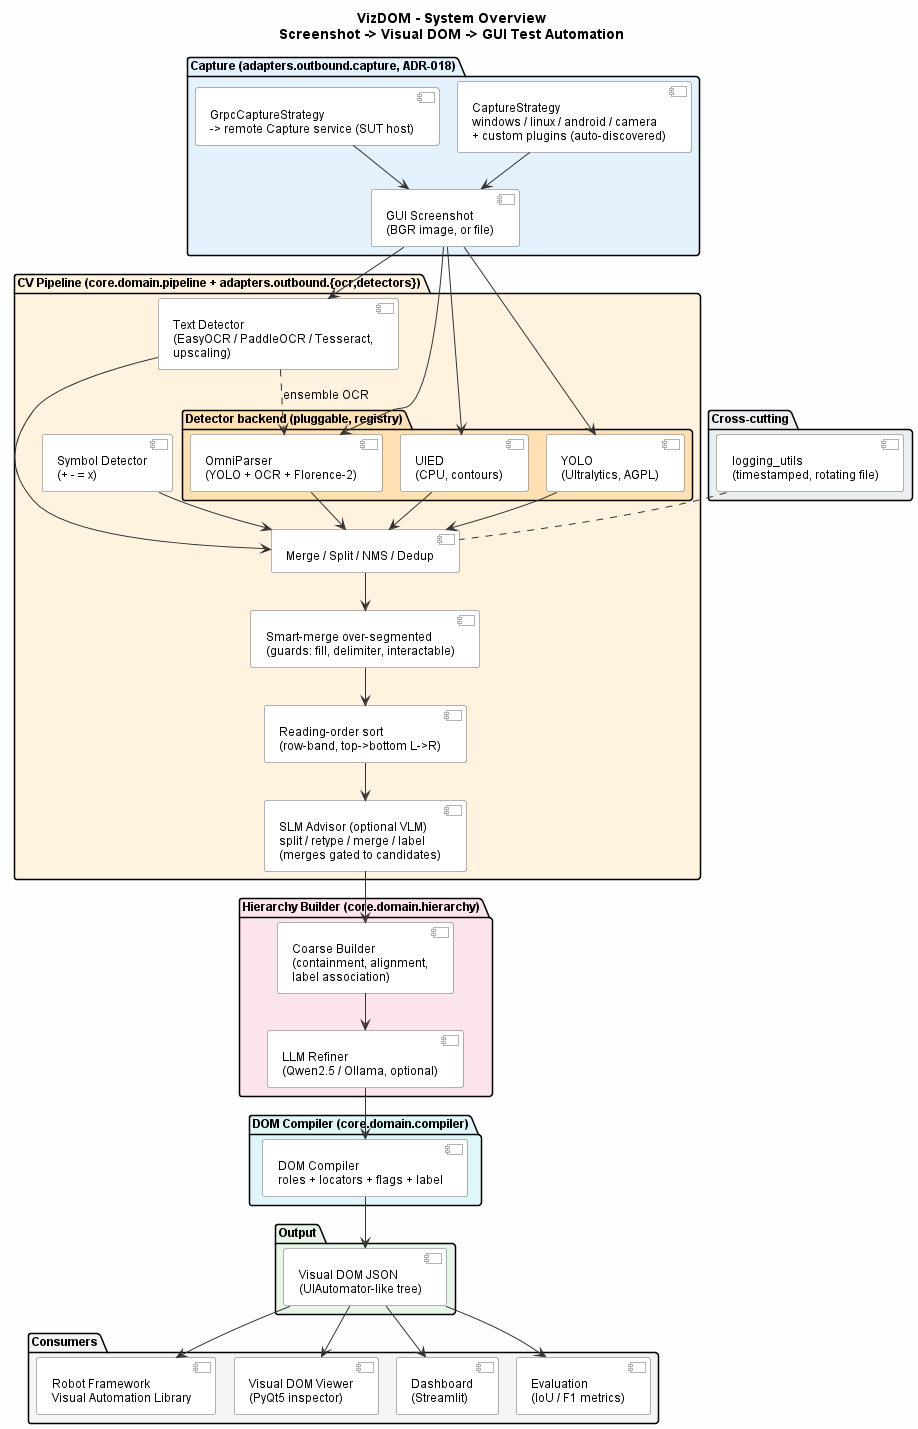
\includegraphics[width=0.62\linewidth]{System_Overview.png}
  \caption{Tổng quan hệ thống: ảnh chụp màn hình $\rightarrow$ Visual DOM
  $\rightarrow$ tự động hóa kiểm thử. Capture cung cấp đầu vào cho CV pipeline;
  detector có thể thay thế và lớp OCR tạo ra các phần tử, sau đó chúng được gộp,
  sắp xếp, tùy chọn tinh chỉnh bằng mô hình nhỏ, tổ chức thành hierarchy và biên
  dịch thành DOM để các công cụ phía sau sử dụng.}
  \label{fig:overview}
\end{figure}

% =====================================================================
\section{Cơ sở lý thuyết và các công trình liên quan}
% =====================================================================

\subsection{Tự động hóa dựa trên accessibility}
UI Automator, Windows UIA và web DOM cung cấp cho test framework một cây gồm các
phần tử có thể tham chiếu \cite{uiautomator,appium}. VizDOM nhắm chính xác đến các
trường hợp cây này không tồn tại hoặc không đáng tin cậy, với mục tiêu
\emph{tổng hợp} một cây tương đương từ pixel.

\subsection{Tự động hóa dựa trên hình ảnh}
Sikuli và các công cụ tương tự \cite{yeh2009sikuli} định vị phần tử bằng template
matching trên ảnh chụp màn hình. Cách tiếp cận này hoạt động khi thiếu dữ liệu
accessibility, nhưng dễ hỏng khi vị trí hoặc giao diện thay đổi, đồng thời không tạo
ra hierarchy có cấu trúc, role hay locator dựa trên text. Ngược lại, VizDOM sinh ra
một cây phần tử đầy đủ.

\subsection{Không gian bài toán phát hiện phần tử GUI}
Phát hiện phần tử trong GUI không giống với object detection trên ảnh tự nhiên;
nghiên cứu nền tảng mà VizDOM kế thừa \cite{xie2020uied} chỉ ra các khó khăn đặc thù
của GUI ở hai cấp độ. Ở cấp độ \emph{phần tử}: (i) \emph{biến thiên nội lớp lớn}
--- cùng một lớp như \code{button} hoặc \code{input\_field} có thể khác nhau đáng
kể về kích thước, hình dạng, màu sắc và phong cách giữa các thiết kế và nội dung;
và (ii) \emph{độ tương đồng liên lớp cao} --- các lớp khác nhau có thể trông gần
như giống hệt nhau (chẳng hạn button và spinner), chỉ được phân biệt bởi một dấu
hiệu rất nhỏ như viền mảnh hoặc glyph nhỏ. Ở cấp độ \emph{GUI}: (iii) widget, hình
ảnh và text xuất hiện đồng thời trong một \emph{hỗn hợp không đồng nhất}, thường nằm
sát nhau; (iv) giao diện thường \emph{dày đặc}, với các phần tử chỉ cách nhau vài
pixel; và (v) ứng dụng đòi hỏi phát hiện vùng với \emph{độ chính xác cao} --- một
bounding box lỏng, dù đủ để nhận diện vật thể trong ảnh, vẫn không đủ để thao tác
hoặc assertion trên control. Những đặc điểm này trực tiếp dẫn đến các bước làm sạch
của VizDOM: bước smart-merge và sắp xếp reading order (Phần~\ref{sec:impl}) được tạo
ra để xử lý phần tử dày đặc, liền kề và bị phân đoạn quá mức; còn ảnh hưởng của quy
ước bounding box trong phần đánh giá (Phần~\ref{sec:eval}) là hệ quả trực tiếp của
yêu cầu độ chính xác cao. Hình~\ref{fig:problemspace} tóm tắt hệ phân loại này.

\paragraph{Khó khăn thứ sáu, đặc thù của kiểm thử: đặt tên cho phần tử không có text.}
Năm đặc điểm phía trên chủ yếu liên quan đến việc \emph{phát hiện} phần tử; trong khi đó, automation còn cần \emph{gọi tên} được phần tử để sử dụng trong locator. Nhiều control GUI hoàn toàn không có text có thể đọc được, chẳng hạn toolbar icon, nút điều khiển cửa sổ, phím toán tử hay button chỉ chứa glyph. Detector có thể xác định vị trí của control một cách chính xác nhưng người viết test vẫn không có giá trị nào để đưa vào locator. Đây là một bài toán độc lập, không phải hệ quả trực tiếp của detection accuracy, và ba cách xử lý mặc định đều có hạn chế. Dùng vị trí thì dễ hỏng khi layout thay đổi, đúng như nhược điểm của các công cụ dựa trên ảnh. OCR thường không trả về gì vì không có text, hoặc tệ hơn là trả về nhiễu từ glyph trang trí. Caption model chỉ đưa ra một \emph{dự đoán}, và thử nghiệm cho thấy dự đoán này có thể thiếu ổn định: hai ảnh chụp cùng một màn hình chỉ khác nhau bởi nhiễu tái mã hóa rất nhỏ ($\leq$7/255 trên mỗi kênh màu) đã khiến caption của icon thay đổi từ ``Maximize'' thành ``Page'' (Phần~\ref{sec:eval}). Vì vậy, VizDOM xem ngữ nghĩa của phần tử không có text là một yêu cầu hạng nhất và xử lý theo nhiều lớp: đọc trực tiếp glyph nếu hình dạng thuộc tập ký hiệu đã biết; giữ label sinh từ caption tách biệt hoàn toàn với text thực sự đọc được; gán tên chuẩn hóa cho các control đã nhận dạng; và dùng grounding dựa trên mô tả như phương án cuối. Cơ chế này được trình bày tại Phần~\ref{sec:impl} và đánh giá tại Phần~\ref{sec:eval}.

\begin{figure}[H]
  \centering
  \includegraphics[width=0.86\linewidth]{Problem_Space.png}
  \caption{Không gian bài toán phát hiện phần tử GUI ở cấp độ phần tử và cấp độ
  GUI (phỏng theo Xie và cộng sự~\cite{xie2020uied}). Các khó khăn này là cơ sở cho
  những bước làm sạch của VizDOM và giải thích ảnh hưởng của quy ước bounding box
  trong phần đánh giá.}
  \label{fig:problemspace}
\end{figure}

\subsection{Không gian giải pháp: cổ điển, deep learning hay kết hợp}
Đối với các phần tử \emph{không phải text}, có hai họ phương pháp cạnh tranh.
Computer vision \emph{cổ điển} tổng hợp edge/contour và region; cách tiếp cận này
không cần huấn luyện và dễ diễn giải, nhưng các đặc trưng thị giác trong thế giới tự
nhiên không ánh xạ tốt sang các hình dạng GUI phẳng, tổng hợp, đồng thời gặp khó
khăn với GUI có nhúng ảnh thật. Detector \emph{deep learning} hồi quy bounding box
--- gồm các họ anchor-based (Faster~R-CNN, YOLO) hoặc thiết kế anchor-free
(CenterNet); chúng có khả năng khái quát tốt nhưng nhạy với định nghĩa anchor,
hyper-parameter và dữ liệu huấn luyện, trong khi box regression có thể không đạt độ
chính xác mà GUI yêu cầu. Kết quả thực nghiệm của nghiên cứu nền tảng
\cite{xie2020uied} cho thấy một phương án \emph{kết hợp} --- dùng đề xuất region cổ
điển để tạo bounding box chính xác cho phần tử không phải text, dùng mô hình deep
learning để phân loại và có một nhánh riêng cho text --- hiệu quả hơn khi chỉ dùng
một trong hai họ. Với \emph{text}, OCR có sẵn (ví dụ Tesseract) là công cụ phổ biến,
nhưng text trong GUI khác text tài liệu (background nhiễu, nằm sát widget), vì vậy
thường cần scene-text model và xử lý chuyên biệt cho GUI.

VizDOM là hiện thực kỹ thuật của câu hỏi ``cổ điển, deep learning hay kết hợp?'':
detector port có thể thay thế cho phép lựa chọn và so sánh trực tiếp baseline cổ
điển (UIED), detector deep learning (YOLO, OmniParser) và phương án hybrid
(Phần~\ref{sec:arch}), trong khi lớp OCR và cơ chế ensemble xử lý nhánh text. Phần
đánh giá (Phần~\ref{sec:eval}) chính là phép so sánh đồng nhất mà cách đặt vấn đề này
đòi hỏi.

\subsection{Phát hiện và grounding phần tử GUI}
Phương pháp detection cổ điển (UIED \cite{xie2020uied}) kết hợp phân tích connected
component/edge với OCR để tìm phần tử text và non-text trên các UI sạch. Các
detector học máy --- họ YOLO \cite{ultralytics} và gần đây là các hệ thống vision
grounding như Microsoft OmniParser \cite{omniparser2024} (detector icon YOLO, mô
hình caption Florence-2 \cite{florence2} và OCR) --- có khả năng định vị và mô tả
phần tử tương tác với độ khái quát tốt. Các mô hình instruction grounding gần đây
(Aria-UI \cite{ariaui2024}) và benchmark grounding (OSWorld-G/Jedi
\cite{osworldg}) nhắm đến bài toán ``với một instruction, hãy chỉ vào phần tử'', bổ
sung cho mục tiêu của VizDOM là sinh ra một cây \emph{đầy đủ} thay vì chỉ một điểm
grounding. VizDOM xem các detector này là những backend có thể hoán đổi, thay vì
phụ thuộc cố định vào một backend.

\subsection{OCR}
Text được trích xuất bằng EasyOCR \cite{easyocr} và/hoặc Tesseract
\cite{tesseract}, kèm upscaling cho text nhỏ; ngoài ra, VizDOM sử dụng OCR như một
tín hiệu \emph{ensemble} cung cấp cho OmniParser nhằm khôi phục những text mà bản
thân detector bỏ sót.

\subsection{Góc nhìn so sánh về hệ sinh thái}
Các hệ thống hiểu GUI gần đây có thể chia thành hai nhóm. \emph{Parser} trả lời câu
hỏi ``trên màn hình có gì?'' bằng cách liệt kê các phần tử (UIED, OmniParser và
VizDOM); \emph{grounder} trả lời ``$X$ nằm ở đâu?'' bằng cách trả về một vị trí duy
nhất cho instruction bằng ngôn ngữ tự nhiên (Aria-UI \cite{ariaui2024}, ELAM-7B
\cite{elam7b} và Jedi/OSWorld-G \cite{osworldg}). Hai nhóm bổ sung cho nhau chứ
không thể thay thế trực tiếp. Bảng~\ref{tab:models} tóm tắt các hệ thống và
Bảng~\ref{tab:capability} đối chiếu khả năng của chúng.

\begin{table}[H]
  \centering\footnotesize
  \caption{Bức tranh tổng quan về các hệ thống hiểu GUI. ``n/v'' = giấy phép chưa
  được xác minh. Các số liệu được trích theo báo cáo của tác giả từng hệ thống.}
  \label{tab:models}
  \begin{tabular}{@{}p{2.4cm}p{2.5cm}p{2.7cm}p{0.8cm}p{2.3cm}p{2.0cm}@{}}
    \toprule
    Hệ thống & Mô hình tiếp cận & Mức chi tiết đầu ra & GPU & Mô hình gốc / kích thước & Giấy phép \\
    \midrule
    VizDOM (đề xuất) & parser (CV + SLM) & cây DOM phân cấp & Không$^\ast$ & pipeline kết hợp & tùy backend \\
    UIED & CV cổ điển & danh sách phần tử phẳng & Không & --- & research \\
    OmniParser V2 & detector + caption & bounding box phẳng có label + khả năng tương tác & Có & YOLOv8 + Florence-2 & AGPL-3.0 / MIT \\
    Aria-UI & vision grounding & một điểm $[0,1000]$ & Có & Aria MoE (3.9B act.) & n/v \\
    ELAM-7B & grounding + đánh giá & điểm + PASSED/FAILED & Có & Molmo-7B-D (Qwen2-7B) & Apache-2.0 \\
    Jedi-3B/7B & vision grounding & một điểm & Có & 3B / 7B & n/v \\
    \bottomrule
  \end{tabular}\\[0.3em]
  {\footnotesize $^\ast$ Chạy trên CPU với backend UIED; backend OmniParser cần GPU để đạt tốc độ thực tế.}
\end{table}

Hai nhận định định hướng thiết kế của VizDOM. Thứ nhất, \emph{không hệ thống nào
trong nhóm so sánh tạo ra hierarchy}: OmniParser chỉ xuất danh sách bounding box có
label dạng phẳng, còn các grounder chỉ xuất một điểm. Thứ hai, tất cả đều hướng đến
\emph{agent} tự trị, có yêu cầu (hoàn thành tác vụ, tính tự chủ) khác căn bản với
\emph{kiểm thử}, nơi cần tính quyết định, khả năng lặp lại, tái sử dụng và chẩn đoán.

\begin{table}[H]
  \centering\footnotesize
  \caption{Ma trận khả năng. ``Có'' = hỗ trợ; ``điểm'' = chỉ trả về điểm;
  ``phẳng'' = danh sách phẳng.}
  \label{tab:capability}
  \begin{tabular}{@{}p{5.2cm}ccccc@{}}
    \toprule
    Khả năng & VizDOM & OmniP. & Aria-UI & ELAM & Jedi \\
    \midrule
    Liệt kê toàn bộ phần tử & Có & Có & Không & Không & Không \\
    Sinh bounding box & Có & Có & điểm & điểm & điểm \\
    Hierarchy / cây DOM & Có & phẳng & Không & Không & Không \\
    Grounding từ instruction NL & qua DOM & Không & Có & Có & Có \\
    Tích hợp đánh giá pass/fail & qua RF & Không & Không & Có & Không \\
    Tái sử dụng cho nhiều action & Có & Có & infer lại & infer lại & infer lại \\
    Chạy không cần GPU & Có & một phần & Không & Không & Không \\
    Đối tượng sử dụng & kiểm thử & agent & agent & kiểm thử HMI & agent \\
    \bottomrule
  \end{tabular}
\end{table}

\subsection{Benchmark và lý do không thể gộp chung}
Bảng~\ref{tab:bench} liệt kê các điểm số do tác giả công bố. Chúng đến từ
\emph{những benchmark khác nhau với độ khó khác nhau} và không được dùng để tạo một
bảng xếp hạng duy nhất; làm như vậy sẽ không hợp lệ về phương pháp luận. Tuy nhiên,
xu hướng chung vẫn đáng chú ý: grounding một bước trên benchmark dễ gần như đã
được giải quyết (82--88\%), nhưng trên benchmark thực tế chỉ còn 40--54\%, còn tỷ
lệ hoàn thành tác vụ agentic đầu-cuối nằm trong khoảng 15\% đến 50\%. Vì vậy,
bottleneck không chỉ nằm ở độ chính xác grounding, mà còn ở \emph{khả năng thực thi
có cấu trúc, tin cậy và lặp lại} --- đúng với lập luận cần một DOM có tính quyết
định trong bối cảnh kiểm thử.

\begin{table}[H]
  \centering\footnotesize
  \caption{Điểm benchmark do tác giả công bố. \textbf{Các benchmark khác nhau ---
  không thể so sánh trực tiếp}; bảng chỉ minh họa khoảng cách giữa bài toán dễ và
  bài toán thực tế, không nhằm xếp hạng.}
  \label{tab:bench}
  \begin{tabular}{@{}p{3.0cm}p{4.4cm}p{3.0cm}p{3.2cm}@{}}
    \toprule
    Hệ thống & Benchmark & Điểm số & Ghi chú \\
    \midrule
    ELAM-7B & AutomotiveUI-Bench-4K & 87.6\% / 78.2\% & grounding / eval; automotive \\
    Aria-UI & ScreenSpot & 82.4\% & dễ, single-step \\
    Jedi-7B & OSWorld-G (564) & 54.1\% & so với UI-TARS-7B 47.5\% \\
    OmniParser V2 & ScreenSpot Pro & 39.5\% & được thiết kế có chủ đích để khó \\
    Aria-UI & OSWorld (agentic) & 15.15\% & tỷ lệ hoàn thành tác vụ đầu-cuối \\
    Jedi-7B + o3 & OSWorld (agentic) & 50.2\% & so với baseline 23\% \\
    \bottomrule
  \end{tabular}
\end{table}

\subsection{Vị trí của VizDOM}
Phát hiện phần tử đang dần trở thành một lớp hàng hóa hóa: một phòng thí nghiệm
công nghiệp (OmniParser) cũng hội tụ về cách phân rã ``CV chịu trách nhiệm geometry,
mô hình bổ sung semantics''. Điều này vừa xác nhận trực giác thiết kế, vừa khiến
detection không còn là yếu tố khác biệt cốt lõi. Những điểm thực sự khác biệt còn
lại là: (i) \emph{xây dựng hierarchy} --- biên dịch containment, alignment và liên
kết label thành một cây có thể truy vấn, điều chưa hệ thống nào trong nhóm so sánh
thực hiện; (ii) \emph{định hướng kiểm thử} --- locator, assertion và keyword Robot
Framework; (iii) \emph{hiệu quả tái sử dụng} --- một lần parse phục vụ nhiều locator
và assertion, trong khi grounder phải infer lại cho từng instruction; và (iv)
\emph{khả năng giải thích} --- cây có thể kiểm tra với các luật matching truy vết
được, thay vì một tọa độ từ black box. Vì vậy, VizDOM xem detector là các backend
có thể thay thế, tận dụng detector mạnh nhất hiện có, còn đóng góp chính nằm ở các
lớp phía trên.

\subsection{Lợi ích của DOM được sinh tự động đối với kiểm thử GUI}
\label{sec:dombenefits}
Các phương pháp tự động hóa được khảo sát ở trên đều đánh đổi theo những trục tương
tự; Bảng~\ref{tab:methods} đối chiếu các phương pháp này. Script dựa trên tọa độ và
hình ảnh không cần nền tảng hỗ trợ, nhưng sẽ hỏng khi layout, theme hoặc độ phân giải
thay đổi và không mang semantics của phần tử. Tự động hóa dựa trên
\emph{accessibility tree} (Appium, Selenium, UIAutomator) là tiêu chuẩn vàng
\emph{khi cây đó tồn tại} --- nhưng nó lại vắng mặt trong canvas Qt/OpenGL render
tùy biến, game, HMI nhúng và mọi màn hình được quan sát qua camera hoặc video
stream. \emph{VLM grounding theo từng instruction} hoạt động mà không cần cây,
nhưng chỉ trả về một tọa độ cho mỗi instruction bằng ngôn ngữ tự nhiên: kết quả
không mang tính quyết định, phải infer lại bằng mô hình lớn ở mỗi action và không
tạo ra cấu trúc có thể tái sử dụng.

Visual DOM được sinh tự động lấp đầy khoảng trống này: nó \emph{tổng hợp} một
artifact tương tự accessibility tree chỉ từ pixel, nhờ đó kiểm thử theo phong cách
cây có thể áp dụng cho các UI vốn không có cây. Cụ thể, cách tiếp cận này mang lại
bốn lợi ích mà test suite cần. (i) \textbf{Tính phổ quát} --- hoạt động ở bất cứ đâu
có pixel (render tùy biến, hệ thống nhúng, máy từ xa, camera), chính là những trường
hợp công cụ dựa trên instrumentation không thể chạy. (ii) \textbf{Locator có
semantics và bền vững} --- role, text, label và quan hệ không gian thay thế tọa độ
pixel dễ hỏng, giúp bài kiểm thử vẫn hoạt động khi phần tử đổi vị trí hoặc phong
cách. (iii) \textbf{Artifact có thể tái sử dụng và kiểm tra} --- một lần parse tạo ra
cây JSON có thể truy vấn, phục vụ nhiều locator và assertion, đồng thời có thể diff,
log và audit; điều này không có ở một lệnh grounding theo từng bước. (iv)
\textbf{Chi phí thấp hơn và có giới hạn} --- perception chỉ chạy một lần trên mỗi
màn hình (và có thể dùng backend CPU), thay vì gọi mô hình lớn cho từng action. Đổi
lại, perception chỉ là xấp xỉ: detection và caption có thể bỏ sót hoặc gán sai label
cho phần tử (recall theo từng loại trong Bảng~\ref{tab:pertype}), vì vậy DOM là bản
tái dựng theo best-effort chứ không phải ground truth. Đây cũng là lý do VizDOM giữ
detector có thể thay thế và báo cáo recall theo từng loại phần tử thay vì chỉ đưa ra
một điểm tổng hợp nổi bật.

\begin{table}[H]
  \centering\footnotesize
  \caption{So sánh các phương pháp kiểm thử GUI theo những yêu cầu quan trọng đối
  với test suite. ``Một phần'' = hỗ trợ một phần.}
  \label{tab:methods}
  \begin{tabular}{@{}p{3.0cm}p{1.7cm}p{1.6cm}p{1.6cm}p{1.6cm}p{1.5cm}@{}}
    \toprule
    Phương pháp & Không cần cây a11y & Custom / camera & Cây có cấu trúc & Locator bền vững & Artifact tái sử dụng \\
    \midrule
    Tọa độ / record--replay & Có & Có & Không & Không & Một phần \\
    Image / template matching & Có & Có & Không & Không & Một phần \\
    Accessibility tree (Appium/UIAutomator) & Không & Không & Có & Có & Có \\
    VLM grounding (theo instruction) & Có & Có & Không & Một phần & Không \\
    \textbf{VizDOM (DOM được sinh)} & Có & Có & Có & Có & Có \\
    \bottomrule
  \end{tabular}
\end{table}

% =====================================================================
\section{Kiến trúc hệ thống}
\label{sec:arch}
% =====================================================================

\subsection{Kiến trúc lục giác: ports and adapters}
VizDOM được tổ chức theo kiến trúc lục giác (Hình~\ref{fig:arch}). Domain core thuần
và chạy cục bộ (điều phối pipeline, logic reading-order và merge, xây dựng hierarchy
thô, biên dịch DOM) chỉ phụ thuộc vào các \emph{port} trừu tượng; adapter cụ thể
được chọn tại runtime. Hệ thống có năm driven port:
\begin{itemize}[leftmargin=1.4em]
  \item \textbf{DetectorPort} --- phát hiện phần tử (UIED, YOLO, OmniParser hoặc
        detector từ xa);
  \item \textbf{OcrPort} --- trích xuất text;
  \item \textbf{RefinerPort} --- review tùy chọn bằng mô hình nhỏ;
  \item \textbf{CapturePort} --- đọc màn hình; và
  \item \textbf{ActuatorPort} --- điều khiển đầu vào.
\end{itemize}
Các driving adapter (CLI, PyQt5 Viewer, Streamlit dashboard và thư viện Robot
Framework) đi vào core thông qua lớp điều phối pipeline.

\begin{figure}[H]
  \centering
  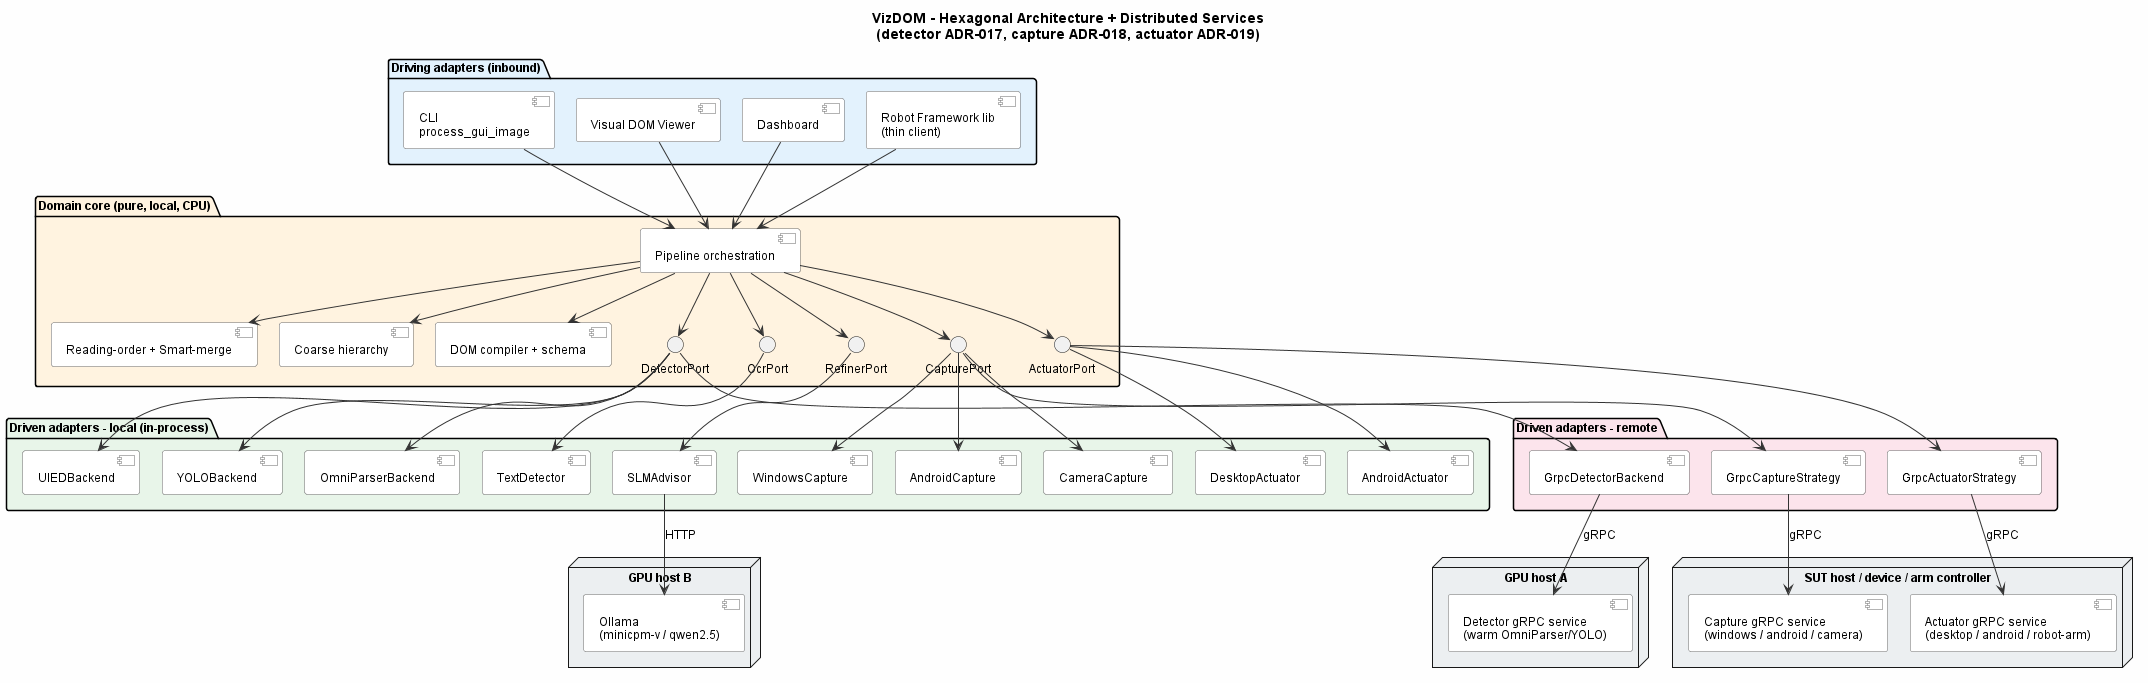
\includegraphics[width=\linewidth]{Architecture.png}
  \caption{Kiến trúc lục giác với các dịch vụ phân tán. Capture, detection và
  actuation là các driven port; mỗi port có adapter chạy trong cùng process và
  adapter gRPC từ xa, nhờ đó dịch vụ có thể lần lượt chạy trên thiết bị cần kiểm
  thử, GPU host và bộ điều khiển cánh tay robot.}
  \label{fig:arch}
\end{figure}

\subsection{Strategy có thể thay thế và cơ chế auto-discovery}
Mỗi port capture, detector và actuator sử dụng cùng một pattern: strategy base
class, registry và cơ chế \emph{auto-discovery} cho plugin người dùng đặt trong thư
mục quy ước (ví dụ \code{plugins/capture/}, \code{plugins/actuator/}). Người dùng
có thể thêm nguồn capture mới hoặc phương thức actuation mới --- camera, capture
card hoặc cánh tay robot --- bằng cách viết một file kế thừa strategy base class.
Registry sẽ nạp plugin ở lần chạy kế tiếp và chọn plugin theo tên trong cấu hình.
Nhờ đó hệ thống có thể mở rộng mà không cần sửa đổi core.

\subsection{Triển khai phân tán qua gRPC}
Do capture phải chạy tại nơi ứng dụng cần kiểm thử hiện diện, detection hưởng lợi từ
GPU, còn actuation xảy ra trên thiết bị hoặc bộ điều khiển vật lý, mỗi port đều có
adapter từ xa được hỗ trợ bởi dịch vụ gRPC \cite{grpc}. Dịch vụ \emph{detector}
kiểu warm-model nạp mô hình nặng một lần rồi phục vụ nhiều client nhẹ; dịch vụ
\emph{capture} cung cấp ảnh chụp màn hình từ thiết bị; dịch vụ \emph{actuator} thực
hiện input trên thiết bị hoặc điều khiển cánh tay robot. Điều quan trọng là gRPC chỉ
là transport, không phải yêu cầu bắt buộc: một lần chạy desktop cục bộ sử dụng
adapter trong process mà không cần server, còn strategy \code{grpc} chỉ được chọn
khi port nằm trên máy khác. Một cấu hình phân tán điển hình là: \emph{capture trên
thiết bị $\rightarrow$ detect trên GPU host $\rightarrow$ actuate trên SUT / bộ điều
khiển cánh tay robot $\rightarrow$ orchestrate trên client}.

\subsection{Contract tọa độ cho actuation}
Detection tạo ra tọa độ theo pixel của ảnh, nhưng vị trí action thực sự được thực
hiện phụ thuộc vào không gian riêng của actuator. Vì vậy, contract actuator của
VizDOM sử dụng tọa độ \emph{chuẩn hóa} trong $[0,1]$ cùng kích thước ảnh nguồn; mỗi
strategy ánh xạ chúng sang không gian thiết bị: desktop nhân với độ phân giải màn
hình, thiết bị Android nhân với độ phân giải input, còn plugin cánh tay robot áp
dụng calibration homography từ pixel ảnh sang tọa độ servo vật lý. Cách này giữ cho
orchestrator và network protocol độc lập với độ phân giải của từng thiết bị.

\subsection{Các quyết định kiến trúc và đánh đổi}
\paragraph{Ports and adapters thay cho layered monolith.} Domain core chỉ phụ thuộc
vào các port trừu tượng, không phụ thuộc detector, nguồn capture hay actuator cụ
thể. Kiến trúc lục giác được chọn vì khả năng kiểm thử (core có thể chạy không cần
I/O) và khả năng thay thế (backend được đổi mà không chạm vào business logic); chi
phí được chấp nhận là một lớp interface và registry cho mỗi port. Đánh đổi này được
xem là hợp lý vì khả năng thay thế là mục tiêu chất lượng quan trọng nhất của dự án.

\paragraph{Phân rã theo định hướng microservice.} Các port không chỉ là những
điểm phân cách nội bộ: mỗi thành phần \emph{detector}, \emph{capture} và
\emph{actuator} đều là một ranh giới dịch vụ hạng nhất, với contract protobuf có
version (\code{protos/*.proto}) và một gRPC server độc lập. Nhờ đó, từng port có
thể được triển khai, scale và nâng cấp như một microservice độc lập. Định hướng
này mang lại các lợi ích của microservice đúng tại nơi bài toán cần đến:
\emph{scale độc lập} (một detector warm-model chạy trên GPU phục vụ nhiều thin
client), \emph{bố trí dị thể} (capture trên thiết bị, detection trên GPU host,
actuation tại SUT hoặc bộ điều khiển cánh tay robot), \emph{cô lập lỗi và tài
nguyên} (detector bị quá tải hoặc gặp sự cố không làm capture đình trệ), và
\emph{khả năng thay thế đa ngôn ngữ} (một dịch vụ có thể được hiện thực lại bằng
bất kỳ ngôn ngữ nào phía sau cùng một contract). Vì vậy, hệ thống được thiết kế
theo định hướng microservice ngay từ đầu --- các service boundary được thiết kế
sẵn chứ không phải bổ sung hồi tố. Tuy nhiên, như trình bày ở quyết định tiếp theo,
các dịch vụ này vẫn có thể thu gọn vào một process khi chỉ cần co-location; nhờ
đó, distribution được áp dụng từng bước thay vì phải trả toàn bộ chi phí ngay từ
đầu.

\paragraph{Tách dịch vụ tùy chọn, không phải microservice luôn hoạt động.} VizDOM là
một \emph{modular monolith} có thể tách từng port thành dịch vụ khi cần, thay vì
phân rã sẵn thành các microservice luôn chạy. Việc phân tán được quyết định bởi
\emph{vị trí vật lý và tài nguyên}, không phải theo xu hướng: capture phải chạy nơi
ứng dụng cần kiểm thử hiện diện, detection hưởng lợi từ GPU và actuation xảy ra trên
thiết bị. Một lần chạy hoàn toàn trong process vẫn là mặc định, tránh chi phí vận
hành (deployment, service discovery, xử lý partial failure) mà thiết kế luôn phân
tán sẽ áp đặt lên trường hợp phổ biến.

\paragraph{gRPC thay cho REST hoặc message broker.} Các port từ xa sử dụng gRPC vì
contract protobuf có kiểu phù hợp với interface ổn định giữa nhiều máy, binary
framing truyền image byte mà không chịu chi phí phình dữ liệu của base64, và mô hình
unary request/response ánh xạ trực tiếp vào các thao tác ``grab a frame'' / ``run
detection'' / ``perform a tap''. REST+JSON sẽ làm tăng kích thước payload ảnh và
mất contract có kiểu; message broker sẽ thêm hạ tầng trái với ràng buộc không dùng
container và áp semantics bất đồng bộ lên các thao tác vốn tự nhiên là đồng bộ.

\paragraph{Mặc định chạy trong cùng process.} Đường gRPC chỉ được chọn khi port nằm
trên máy khác; một lần chạy desktop cục bộ không phải trả chi phí network,
serialization hay vòng đời server. Điều này giữ cho trường hợp đơn giản vẫn đơn
giản, đồng thời cho phép trường hợp phân tán sử dụng \emph{cùng} codebase; đây là cơ
chế cụ thể hiện thực mục tiêu chất lượng về khả năng triển khai.

% =====================================================================
\section{Hiện thực}
\label{sec:impl}
% =====================================================================

\subsection{CV pipeline}
Phép biến đổi cốt lõi là \code{VisualDOMPipeline.process()}
(Hình~\ref{fig:pipeline}). Pipeline gồm các giai đoạn sau:
\begin{enumerate}[leftmargin=1.6em]
  \item \textbf{Thu nhận và chuẩn bị.} Ảnh chụp màn hình được lấy qua capture
        strategy hoặc từ file, tùy chọn hiệu chỉnh trong ``camera mode'', rồi tính
        scale factor theo độ phân giải.
  \item \textbf{Phát hiện text.} OCR engine (EasyOCR/PaddleOCR/Tesseract) kết hợp
        upscaling sinh ra các phần tử text.
  \item \textbf{Phát hiện phần tử.} Một detector backend có thể thay thế được chạy:
        UIED (phân tích contour trên CPU), YOLO, OmniParser (phát hiện icon bằng
        YOLO + caption Florence-2 + OCR) hoặc hybrid. Kết quả detection được chuẩn
        hóa về dạng \code{UIElement} chung.
  \item \textbf{Merge / split / loại trùng.} Text và phần tử được merge dựa trên
        containment/IoU, split theo vị trí text, rồi rút gọn bằng non-maximum
        suppression theo từng type và giữa các type.
  \item \textbf{Smart-merge cho over-segmentation.} Các bounding box rời rạc nhưng
        thuộc cùng một phần tử logic (button nhiều dòng, dòng text bị tách) được
        merge dưới các guard --- ngưỡng fill-ratio, kiểm tra delimiter và quy tắc
        ``tối đa một thành phần có thể tương tác'' --- nhằm tránh gộp nhầm các
        control khác nhau.
  \item \textbf{Sắp xếp reading order.} Các phần tử được sắp theo thứ tự từ trên
        xuống dưới, từ trái sang phải bằng heuristic row-band.
  \item \textbf{Review tùy chọn bằng SLM/VLM.} Mô hình nhỏ được phục vụ qua Ollama
        có thể split, gán lại type, merge và \emph{gán label} cho các phần tử đáng
        ngờ; thao tác merge chỉ được phép trên các candidate đã được geometry phê
        duyệt trước, để mô hình không thể gộp các control không liên quan.
  \item \textbf{Hierarchy và output.} Builder thô suy luận containment, nhóm
        alignment và liên kết label; DOM compiler sinh role, interaction flag,
        nhiều locator và label dễ đọc cho con người.
\end{enumerate}

\begin{figure}[H]
  \centering
  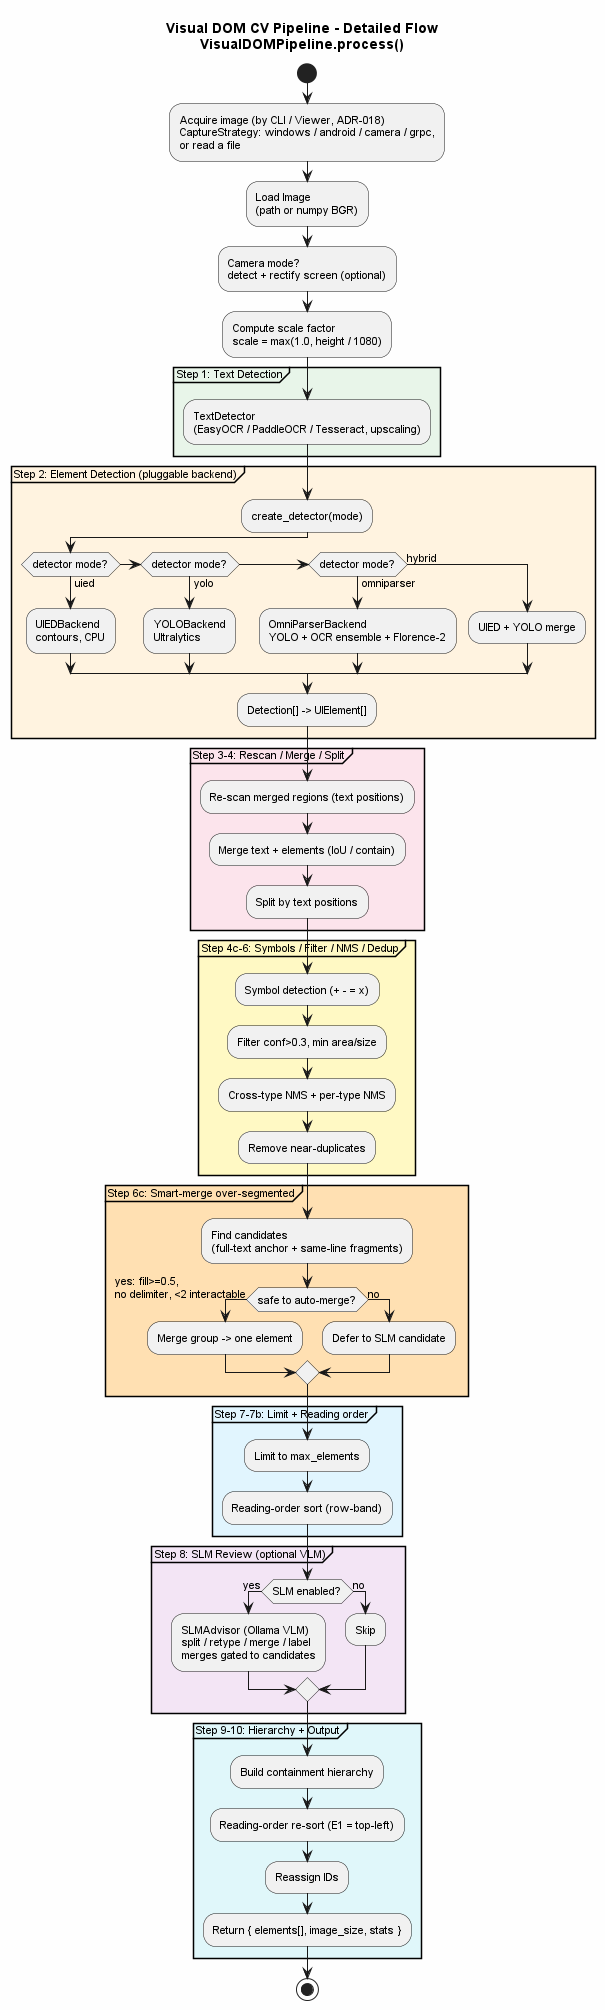
\includegraphics[height=0.86\textheight,width=\linewidth,keepaspectratio]{CV_Pipeline_Detail.png}
  \caption{Control flow chi tiết của \code{VisualDOMPipeline.process()}: thu nhận,
  OCR, detection có thể thay thế, làm sạch, smart-merge, reading-order, review tùy
  chọn bằng mô hình nhỏ và sinh hierarchy/DOM.}
  \label{fig:pipeline}
\end{figure}

\subsection{Các quyết định thiết kế pipeline}
Hình dạng của pipeline xuất phát từ một số quyết định chính, mỗi quyết định nhằm
xử lý một failure mode đã quan sát được:
\begin{itemize}[leftmargin=1.4em]
  \item \textbf{Detector có thể thay thế, không phụ thuộc một mô hình duy nhất.}
        Chất lượng detection thay đổi theo phong cách UI và phần cứng sẵn có; một
        interface ổn định \code{detect(image)} cho phép baseline CPU (UIED) và mô
        hình grounding dùng GPU (OmniParser) cùng tồn tại, được so sánh trực tiếp,
        đồng thời cho phép thay detector giấy phép AGPL bằng detector giấy phép
        permissive mà không sửa pipeline. Đánh đổi: phải duy trì từ hai code path
        trở lên.
  \item \textbf{OCR ensemble.} Detector học máy định vị tốt phần tử tương tác nhưng
        có thể bỏ sót text nhỏ; đưa thêm một lượt OCR có upscaling vào detector giúp
        khôi phục các từ bị bỏ sót (gap-fill de-duplication). Đánh đổi: lượt OCR thứ
        hai làm tăng thời gian, nên được thiết kế tùy chọn.
  \item \textbf{Smart-merge dựa trên luật và có guard \emph{trước} mô hình.}
        OmniParser có xu hướng over-segment (một button nhiều dòng thành nhiều
        bounding box). Merge fragment theo fill-ratio, delimiter và guard ``tối đa
        một thành phần có thể tương tác'' có tính quyết định, rẻ và dễ giải thích,
        đồng thời tránh gộp nhầm các control khác nhau. Đánh đổi: các threshold cần
        tinh chỉnh thủ công.
  \item \textbf{Tinh chỉnh bằng mô hình nhỏ, có gating.} LM/VLM nhỏ chỉ review các
        phần tử đáng ngờ (split / gán lại type / merge / label), và thao tác merge
        bị giới hạn trong các candidate đã được geometry phê duyệt. Vì vậy, mô hình
        xác suất không thể gộp các control không liên quan. Đánh đổi: phát sinh phụ
        thuộc mô hình --- do đó đây là bước tùy chọn và hệ thống vẫn suy giảm mềm
        khi mô hình vắng mặt.
  \item \textbf{Geometry do CV đảm nhiệm, semantics do mô hình đảm nhiệm.} Pipeline
        không cho phép language model sinh tọa độ; mô hình chỉ sở hữu label và type.
        Cách phân chia trách nhiệm này --- cũng được xác nhận độc lập bởi thiết kế
        của OmniParser --- giữ độ chính xác không gian có tính quyết định và dùng mô
        hình tại nơi nó phát huy thế mạnh.
\end{itemize}

\subsection{Các detector backend có thể thay thế}
Detector hiện thực interface chung \code{DetectorBackend}
(\code{detect(image)} $\rightarrow$ \code{List[Detection]}, \code{is\_available()})
và được khởi tạo bởi registry factory. UIED là baseline CPU không yêu cầu dependency
mô hình; YOLO và OmniParser là các backend học máy; backend gRPC chuyển tiếp yêu cầu
đến dịch vụ warm-model từ xa. Trong thực tế, OmniParser phân tách các control nằm
sát nhau (ví dụ các nút máy tính) tốt hơn UIED nhưng có xu hướng over-segment, dẫn
đến nhu cầu smart-merge dựa trên luật và bước tinh chỉnh mô hình nhỏ có guard như
trình bày ở trên.

\subsection{Từ detection đến DOM}
Coarse hierarchy builder liên kết label với control (ví dụ field và caption của
field), nhóm các phần tử thẳng hàng và lồng nhau theo containment. Sau đó, DOM
compiler sinh ra cây JSON tương tự UI Automator: mỗi node chứa id, bounds, center,
role, visual type, interaction flag (clickable/editable/scrollable), text và label
tùy chọn, cùng nhiều \emph{locator} (theo id, text, hint, role và quan hệ không
gian).


\subsection{Văn bản nguyên bản, nhãn ngữ nghĩa và nhận dạng ký hiệu}
Hai bước tinh chỉnh giúp tách biệt nội dung được \emph{đọc} khỏi nội dung được
\emph{suy luận}. Trước hết, DOM phân biệt \code{text} --- nội dung nguyên bản được
đọc từ pixel bằng OCR --- với \code{label} --- tên ngữ nghĩa của phần tử, được xác
định theo thứ tự ưu tiên \emph{label liên kết ở lân cận $>$ caption của detector
$>$ text của chính phần tử}. Sự phân biệt này rất quan trọng vì caption model tạo
ra dự đoán chứ không trực tiếp đọc nội dung: hai ảnh capture nhìn gần như hoàn toàn
giống nhau, chỉ khác bởi nhiễu tái mã hóa không thể nhận biết bằng mắt
($\leq$7/255 trên mỗi channel), đã khiến caption của cùng một icon thay đổi từ
``Maximize'' thành ``Page''. Việc không đưa caption vào \code{text} giúp locator
chỉ phụ thuộc vào những gì thực sự xuất hiện trên màn hình.

Thứ hai, các control chỉ chứa glyph (các phím toán tử
\code{+ - = $\times$ $\div$}, các nút điều khiển cửa sổ) thường không thể được
nhận dạng bằng OCR. Chúng cũng từng làm thất bại symbol detector dựa trên luật:
các projection heuristic không hoạt động ổn định trên glyph thật của phím và nhầm
hình vuông rỗng của nút maximize thành dấu ``+''. Giai đoạn được thiết kế lại nhận
biết các glyph này bằng \emph{template matching}: glyph được crop theo đúng
bounding box của nó và chuẩn hóa theo scale; các hình outline rỗng được loại bỏ
theo cấu trúc; sau đó candidate được so khớp với các template render từ font bằng
Dice score, với acceptance threshold riêng cho từng ký hiệu.

Một ảnh capture thứ hai --- cùng ứng dụng nhưng được render bằng theme có nét glyph
dày hơn --- cho thấy một failure mode tinh vi hơn: bước \emph{chọn phương án nhị
phân hóa} đã chọn sai. Adaptive threshold tạo ra một \emph{artefact dạng vòng}
(glyph xuất hiện như một lỗ rỗng bên trong một khối), nhưng candidate này lại đạt
điểm cao nhất theo density heuristic dùng để chọn giữa các phương án binarization.
Vì vậy, dấu ``$\times$'' nét dày bị match thành template dấu chấm đặc, còn
``$\div$'' và ``$-$'' không match được gì. Giai đoạn này hiện chấm điểm
\emph{mọi} candidate nhị phân hóa --- cả hai polarity và adaptive threshold ---
bằng template matching, đồng thời bổ sung size gate cho dấu ``.'' và các template
dùng font đậm.

Việc mở rộng đánh giá đã buộc phải có một vòng sửa thứ ba, sâu hơn: một similarity
score đơn thuần không thể cho biết ``đây hoàn toàn không phải là ký hiệu''. Trên
tập 130 trường hợp đã gán nhãn --- bốn kiểu render thực tế của cùng một ứng dụng
(hai bố cục keypad, display scaling 100\% và 125\%, theme tối và sáng), bao gồm
cả mọi phím bắt buộc phải bị \emph{từ chối} --- template matcher chỉ đạt 51/130.
Sau khi được chuẩn hóa về một patch cố định, một phím chữ như ``mod'', icon
backspace hoặc một chữ số có thể biến thành vệt giống thanh và vượt threshold của
``$-$'' hoặc ``$=$''; đồng thời một candidate binarization \emph{suy giảm} làm
mất component --- chẳng hạn hai chấm của ``$\div$'' hoặc thanh thứ hai của
``$=$'' --- đôi khi lại được chấm cao hơn cách đọc trung thực từ candidate tốt hơn.

Thiết kế cuối cùng phân loại dựa trên \emph{cấu trúc connected component}:
``$\div$'' phải gồm một thanh ngang rộng với một chấm ở trên và một chấm ở dưới,
``$=$'' phải có đúng hai thanh đặc xếp chồng, còn ``$+$'' phải là một dấu thập cân
giữa với bốn góc rỗng. Template chỉ còn đóng vai trò bằng chứng hỗ trợ. Các
candidate binarization được xếp hạng theo \emph{mức độ đặc hiệu}: kết quả giải
thích được nhiều component hơn sẽ thắng, vì quá trình suy giảm chỉ có thể làm mất
cấu trúc chứ không thể tự tạo thêm cấu trúc hợp lệ. Glyph không khớp cấu trúc nào
sẽ bị từ chối. Kết quả đạt \textbf{130 trên 130} trên cả bốn kiểu render và được
giữ lại như một regression test dựa trên dữ liệu; trên tập tổng hợp, cùng thay đổi
này loại bỏ thêm ba false positive và khôi phục hai glyph ``\%'' từng bị bỏ sót.
Kết quả được đưa vào \code{text} --- vì ký hiệu là nội dung được đọc trực tiếp --- nên một
phím toán tử vẫn có thể được điều khiển bằng \code{text="+"} ngay cả khi caption
bị nhiễu. Khi kết quả đủ tin cậy, hệ thống còn gán một \emph{label chuẩn hóa}
(``$\div$''$\rightarrow$Divide, ``$\times$''$\rightarrow$Multiply), thay thế
caption dễ nhầm trên các phím toán tử; các control trên title bar vẫn giữ caption vì
đó mới là tên thực của chúng. Tập ký hiệu được nhận dạng và mức độ nghiêm ngặt có
thể cấu hình trong section \code{symbols}.

\subsection{Thư viện Visual Automation cho Robot Framework}
Deliverable thứ hai là thư viện Robot Framework \cite{robotframework}, hoạt động
như một orchestrator mỏng phía trên các port capture và actuator. Một số keyword
đại diện:
\begin{itemize}[leftmargin=1.4em]
  \item \emph{Capture / phân tích}: \code{Capture Screen}, \code{Dump Visual DOM},
        \code{Load Visual DOM}, \code{Bring App To Front};
  \item \emph{Truy vấn}: \code{Get Visual Element}, \code{Get Element Property},
        \code{Get Element Text}, \code{Get Element Label}, \code{Get Element Center};
  \item \emph{Action}: \code{Click Visual}, \code{Type Text Visual},
        \code{Press Key}, \code{Scroll Visual}, \code{Drag And Drop Visual};
  \item \emph{Assertion / wait}: \code{Visual Should Exist},
        \code{Visual Should Not Exist}, \code{Wait Until Visual Appears},
        \code{Wait Until Visual Disappears}.
\end{itemize}
Locator hỗ trợ \code{id=}, \code{text=}, \code{hint=}, \code{role=}, các quan hệ không gian (\code{within=}, \code{right\_of=}, \code{below=}, \dots) và \code{desc=} (Phần~\ref{sec:desc}). Nhiều locator trong cùng một chuỗi được kết hợp theo điều kiện \emph{and}; ngược lại, dấu phân cách \code{||} biểu diễn một \emph{fallback chain} có thứ tự, được thử từ trái sang phải cho đến khi một phương án resolve chính xác thành một phần tử:

\begin{quote}\small
\code{Click Visual~~~~text=Save || desc="save button in the toolbar"}
\end{quote}

\noindent Một phương án bị bỏ qua không chỉ khi không tìm thấy kết quả, mà cả khi kết quả \emph{mơ hồ}; locator trả về nhiều phần tử cũng không thể sử dụng an toàn như locator không tìm thấy phần tử. Khi cả chain thất bại, thông báo lỗi liệt kê từng phương án đã thử cùng nguyên nhân tương ứng để vẫn có thể debug. Do các phương án có thứ tự, người viết test cũng kiểm soát được chi phí: lookup xác định bằng \code{text=} gần như không tốn chi phí và được chạy trước; \code{desc=} chỉ được sử dụng sau khi phương án trước thất bại và có thể gọi model. Khi một phương án phía sau thành công, thư viện phát warning và chỉ rõ phương án nào đã thất bại. Đây là tín hiệu cho thấy locator chính đã lỗi thời, đồng thời là đầu vào có thể đo lường cho cơ chế self-healing locator được liệt kê trong phần công việc tương lai (ADR-024).

Action phân giải locator thành phần tử, chuyển center sang tọa độ chuẩn hóa rồi ủy quyền cho actuator. Nhờ vậy, cùng một bài kiểm thử có thể chạy cục bộ, qua gRPC hoặc với cánh tay robot mà không cần thay đổi.

\begin{figure}[H]
  \centering
  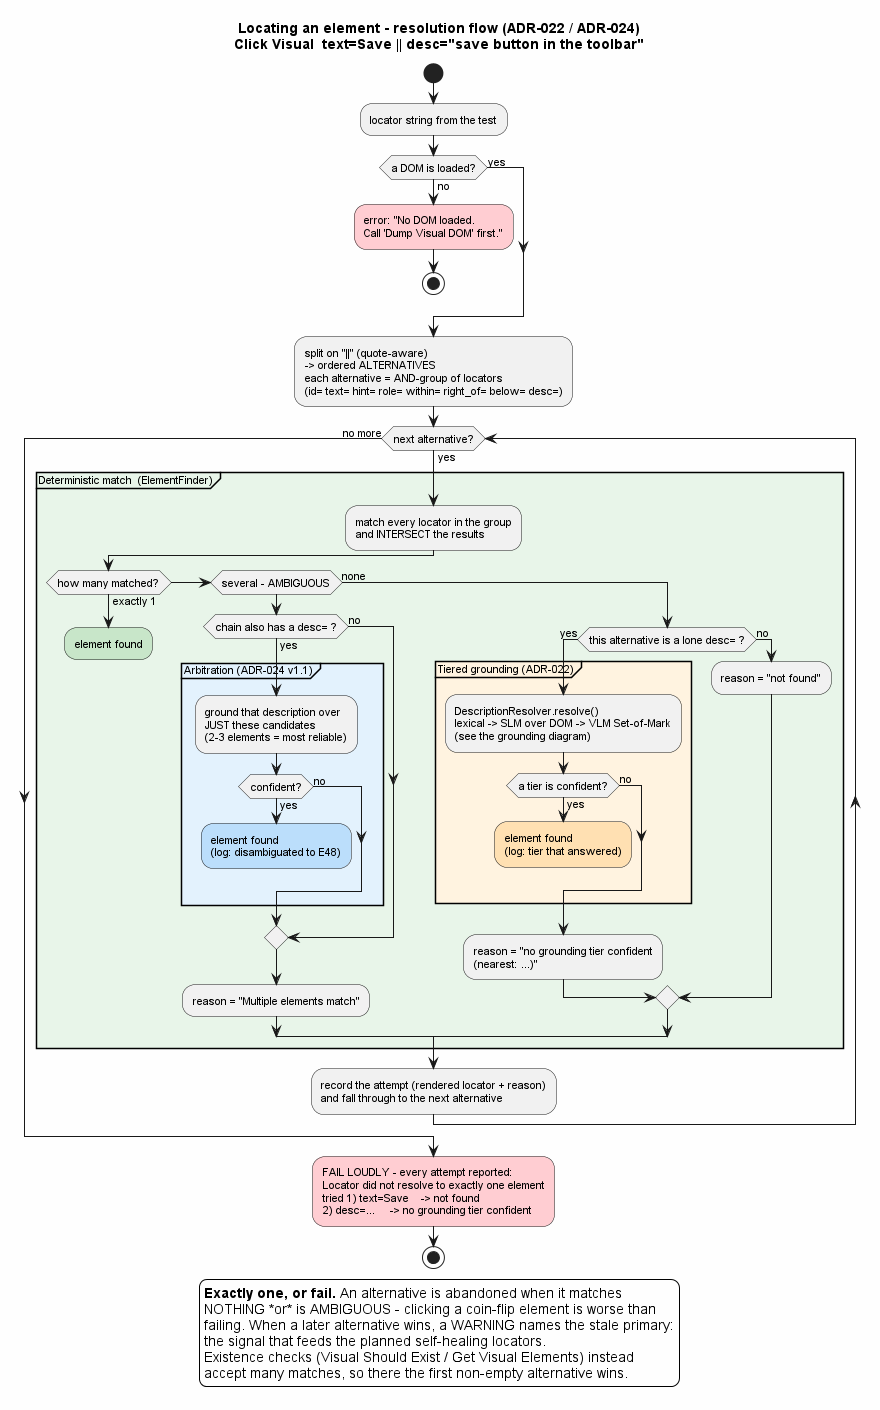
\includegraphics[width=0.72\linewidth]{Locator_Resolution.png}
  \caption{Quá trình phân giải locator về đúng một phần tử. Các phương án được
  phân tách bằng \code{||} và thử theo thứ tự; một phương án bị bỏ qua nếu
  \emph{không khớp phần tử nào} hoặc cho kết quả \emph{mơ hồ}. Nếu trong chain
  có \code{desc=}, nó có thể trước hết dùng để phân xử giữa các candidate mơ hồ
  (ADR-024); nếu chỉ có một description locator, quá trình sẽ tăng dần qua các
  grounding tier (Hình~\ref{fig:descgrounding}). Khi cả chain thất bại, hệ thống
  báo lại toàn bộ các phương án đã thử cùng nguyên nhân tương ứng.}
  \label{fig:locatorflow}
\end{figure}

\begin{figure}[H]
  \centering
  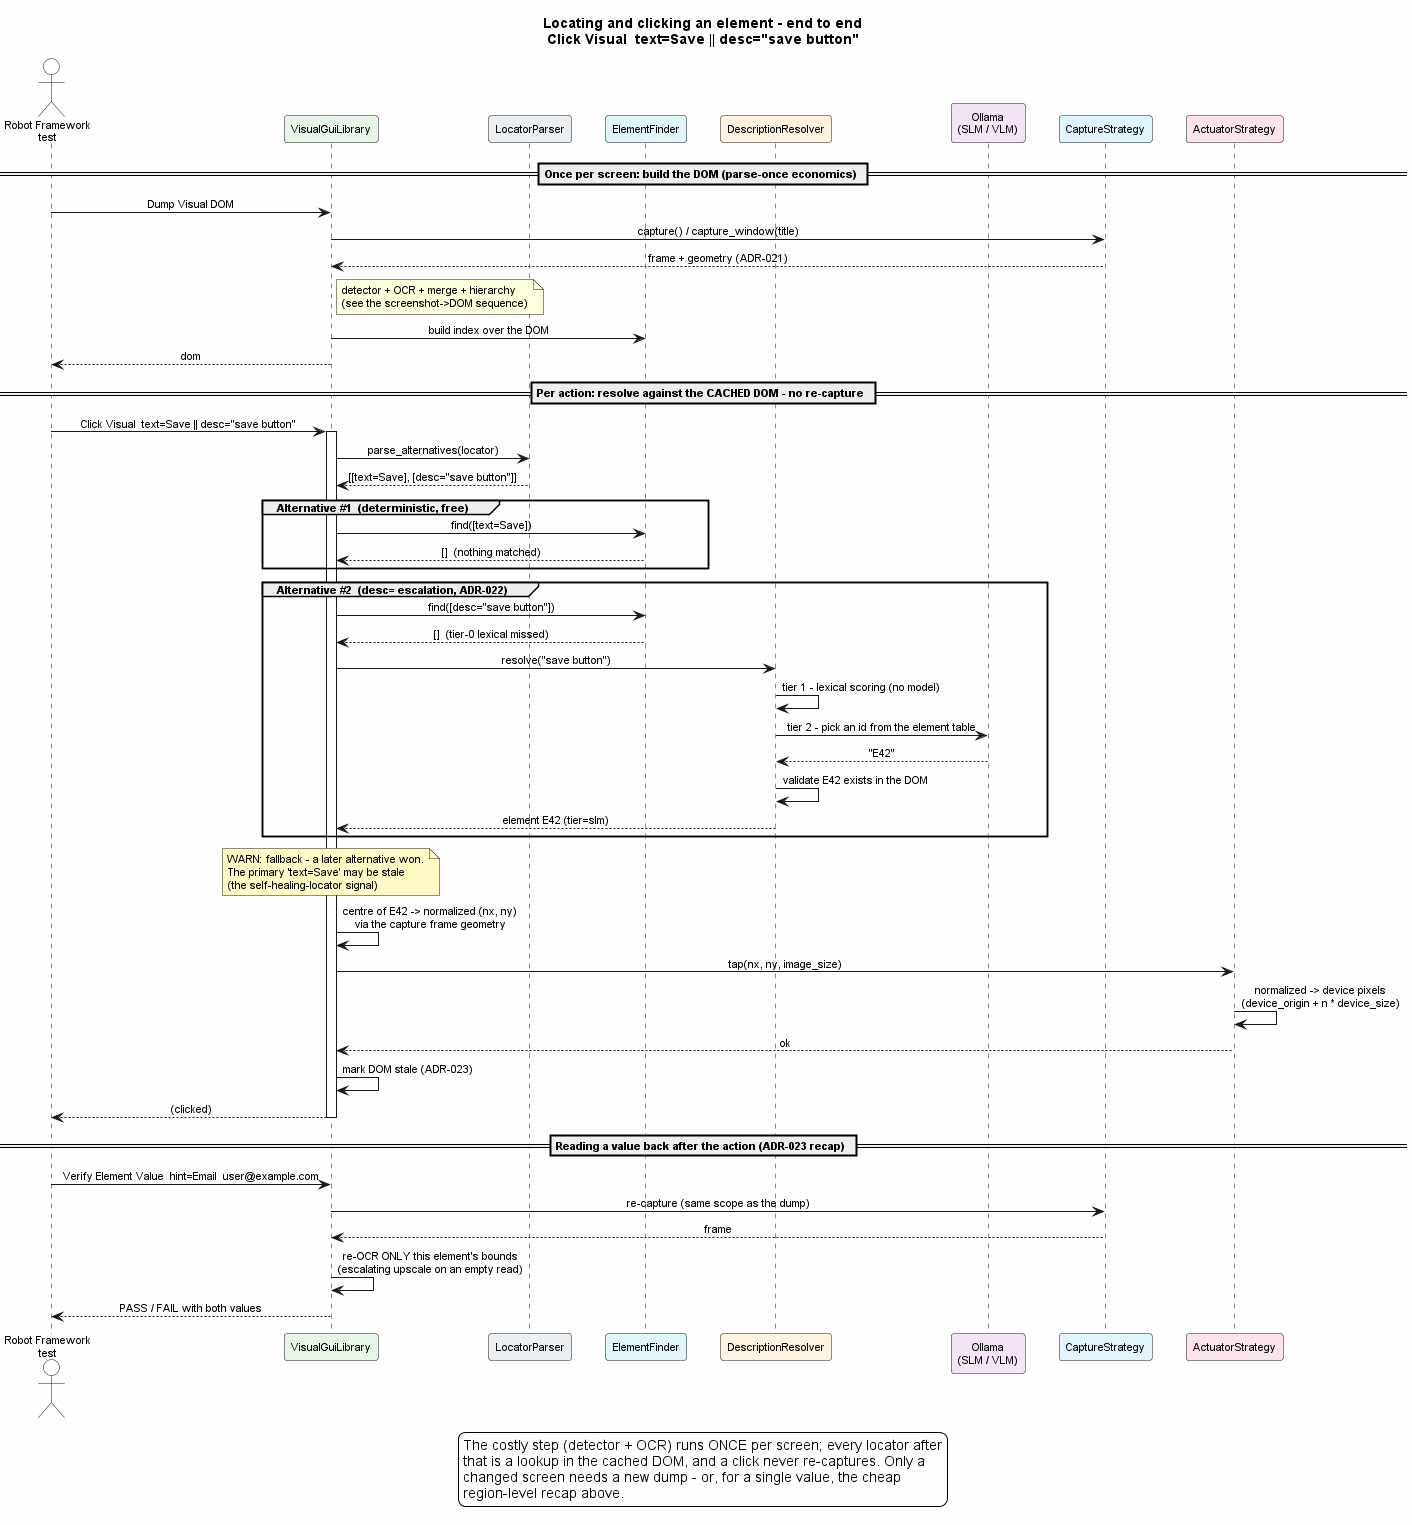
\includegraphics[width=\linewidth]{Locator_Sequence.png}
  \caption{Luồng tương tác đầu-cuối cho một action. Bước perception tốn chi phí
  chỉ chạy \emph{một lần} cho mỗi màn hình; các locator sau đó chỉ là lookup trên
  DOM đã cache và thao tác click không cần capture lại. Tâm của phần tử được chuẩn
  hóa dựa trên geometry của capture frame trước khi actuator ánh xạ sang tọa độ
  pixel của thiết bị (Phần~\ref{sec:impl}); khi cần đọc lại một giá trị, hệ thống
  dùng region-level recapture thay vì chạy lại toàn bộ detector.}
  \label{fig:locatorseq}
\end{figure}

\subsubsection*{Nhắm đúng ứng dụng}
Một yêu cầu đúng đắn ít hiển nhiên hơn xuất phát từ chính hai lựa chọn thiết kế
phía trên: hệ thống chụp \emph{toàn bộ màn hình} và thao tác bằng \emph{tọa độ
tuyệt đối}. Cả hai đều âm thầm cho kết quả sai khi ứng dụng đang kiểm thử không
phải foreground window. Nếu một cửa sổ khác che phía trên, ảnh chụp sẽ tạo ra
Visual DOM của nhầm ứng dụng; một click tại tọa độ vốn đúng với screenshot sẽ rơi
vào bất kỳ cửa sổ nào đang chiếm điểm đó, còn văn bản được nhập vào nơi đang giữ
keyboard focus. DOM không thể chỉ ra sai sót này: tọa độ vẫn nhất quán với
screenshot, và screenshot cũng nhất quán với thời điểm được chụp.

Vì vậy, hệ thống xem ``đưa ứng dụng lên foreground'' là một capability tường minh
của cả hai driven port (\code{focus\_target()}, ADR-021), với implementation
riêng theo nền tảng: chuỗi xử lý Win32 trên Windows --- restore, gắn vào input
queue của foreground thread, gửi một modifier giả lập và tạm đặt top-most ---
\code{wmctrl}/\code{xdotool} trên X11, và \code{am start} để đưa activity về
trạng thái resumed trên Android. Hai đặc tính giúp cơ chế này đáng tin cậy thay vì
chỉ tiện dụng. Thứ nhất, thành công luôn được \emph{xác minh}: strategy đọc lại
foreground window thực tế sau thao tác, vì hệ điều hành có thể từ chối yêu cầu một
cách hợp lệ --- chẳng hạn foreground lock của Windows --- và việc lạc quan trả về
``true'' sẽ biến lần từ chối đó thành một screenshot sai khó giải thích. Thứ hai,
focus được thực hiện \emph{tại nơi màn hình tồn tại}: trong cấu hình phân tán, thao
tác này được truyền bằng một \code{Focus} RPC riêng đến capture service và
actuator service, vì client trên máy khác không thể đưa một cửa sổ không thuộc máy
đó lên foreground. Trường hợp mơ hồ được xem là lỗi chứ không phải cơ hội để đoán:
nếu window title khớp nhiều cửa sổ, hệ thống trả về danh sách ứng viên thay vì
điều khiển một cửa sổ tùy ý. Cơ chế được cung cấp theo hai mức có chủ ý --- một
keyword tường minh làm test thất bại khi không focus được, và một cờ cấu hình
opt-in đưa target lên foreground trước mỗi lần capture nhưng chỉ ghi warning ---
vì đưa cửa sổ lên foreground bản thân nó là một action có thể làm biến mất UI tạm
thời; do đó không bao giờ được ngầm thực hiện như một phần của thao tác đọc.

Hình~\ref{fig:seq} mô tả tương tác đầu-cuối của một chu kỳ từ ảnh chụp màn hình đến DOM.

\begin{figure}[H]
  \centering
  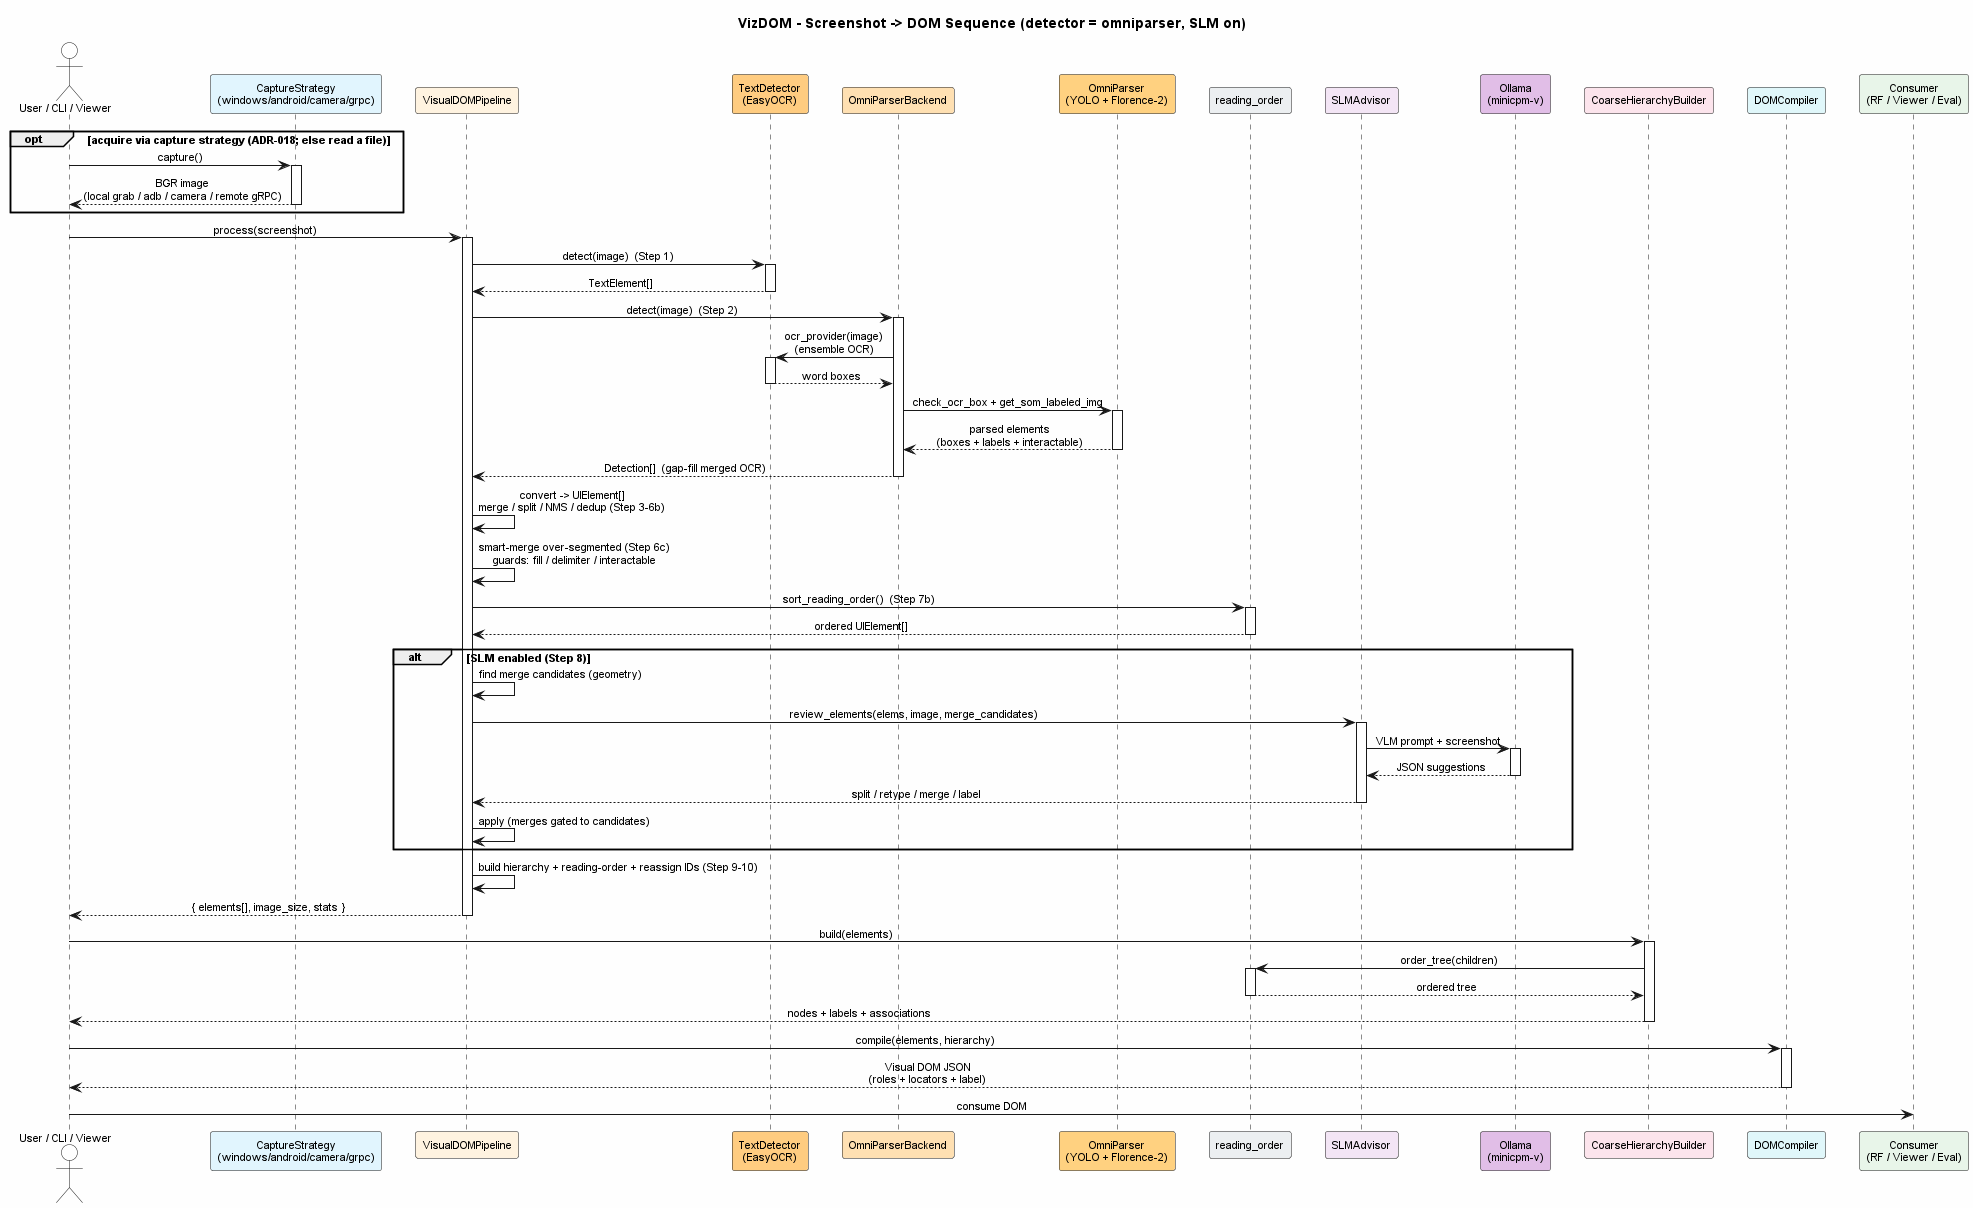
\includegraphics[width=\linewidth]{Sequence_Diagram.png}
  \caption{Trình tự của một chu kỳ từ ảnh chụp màn hình đến DOM (detector =
  OmniParser, bật SLM): capture tùy chọn, OCR, detection với OCR ensemble, làm sạch,
  reading-order, review tùy chọn bằng mô hình nhỏ, xây dựng hierarchy và biên dịch
  DOM cho consumer.}
  \label{fig:seq}
\end{figure}


\subsection{Định vị dựa trên mô tả: grounding phân tầng trên DOM}
\label{sec:desc}
Property locator có tính quyết định nhưng lại dễ trở nên mong manh đúng tại những
điểm perception yếu nhất: một icon có caption không ổn định hoặc một phím có kết
quả OCR nhiễu sẽ không thể được tìm bằng \code{text=}. Vì vậy, locator
\code{desc=} cho phép tester mô tả \emph{ý định} --- ví dụ
\code{desc="settings button"} --- và đưa mô hình grounder
(Phần~\ref{sec:dombenefits}) vào hệ thống parser, trong khi DOM vẫn được giữ làm
source of truth. Quá trình phân giải được nâng dần qua các tier có thể cấu hình;
mỗi tier rẻ hơn và có tính quyết định cao hơn tier kế tiếp, và chuỗi dừng ngay khi
tìm được một kết quả đủ tin cậy. Luồng phân giải này được minh họa ở
Hình~\ref{fig:descgrounding}:
\begin{enumerate}[leftmargin=1.6em,label=(\roman*)]
  \item Tier \emph{lexical} không dùng mô hình, chấm điểm mức trùng khớp token và
        synonym với \code{label}/\code{text}/\code{hint}, kết hợp các từ chỉ role;
        kết quả chỉ được chấp nhận khi vượt score floor và có margin đủ lớn so với
        candidate đứng thứ hai --- nếu hòa điểm, hệ thống chuyển lên tier kế tiếp
        thay vì đoán;
  \item Tier \emph{SLM-over-DOM} cung cấp cho một text model nhỏ
        (temperature 0) bảng phần tử rút gọn và kiểm tra id trả về với DOM; các id
        do mô hình hallucinate sẽ bị từ chối;
  \item Tier \emph{VLM} tùy chọn sử dụng Set-of-Mark prompting: các bounding box
        candidate được đánh số trên ảnh chụp màn hình và mô hình chọn một số. Nhờ
        đó, câu trả lời luôn ánh xạ tới một phần tử DOM \emph{theo thiết kế}, tránh
        coordinate regression vốn kém ổn định.
\end{enumerate}
Hai phát hiện thực nghiệm đã định hình thiết kế này. Trước hết, các từ chỉ vị trí
như ``top right'' được áp dụng bằng \emph{geometry} trước khi gọi bất kỳ mô hình
nào: một mô hình 3B từng tự tin nhận nhầm phần tử ở góc trên bên trái thành ``top
right'', nên vị trí không bao giờ được giao hoàn toàn cho mô hình. Thứ hai, tính
quyết định là một policy chứ không phải kết quả ngẫu nhiên: chuỗi tier được cấu
hình theo từng session (CI có thể cố định chỉ dùng tier lexical), kết quả phân giải
được cache theo từng màn hình và mỗi hit đều ghi nhận tier đã trả lời. Nhờ vậy,
hiệu quả kinh tế của cách tiếp cận ``parse một lần, chỉ grounding phần long tail''
có thể được đo lường. Trong một session thực tế với ứng dụng máy tính, chuỗi này
phân giải đúng 5/5 mô tả thử nghiệm (các cách diễn đạt lại được xử lý bởi tier SLM)
và từ chối chính xác một mô tả vô nghĩa bằng cách trả về danh sách candidate
(ADR-022).

\begin{figure}[H]
  \centering
  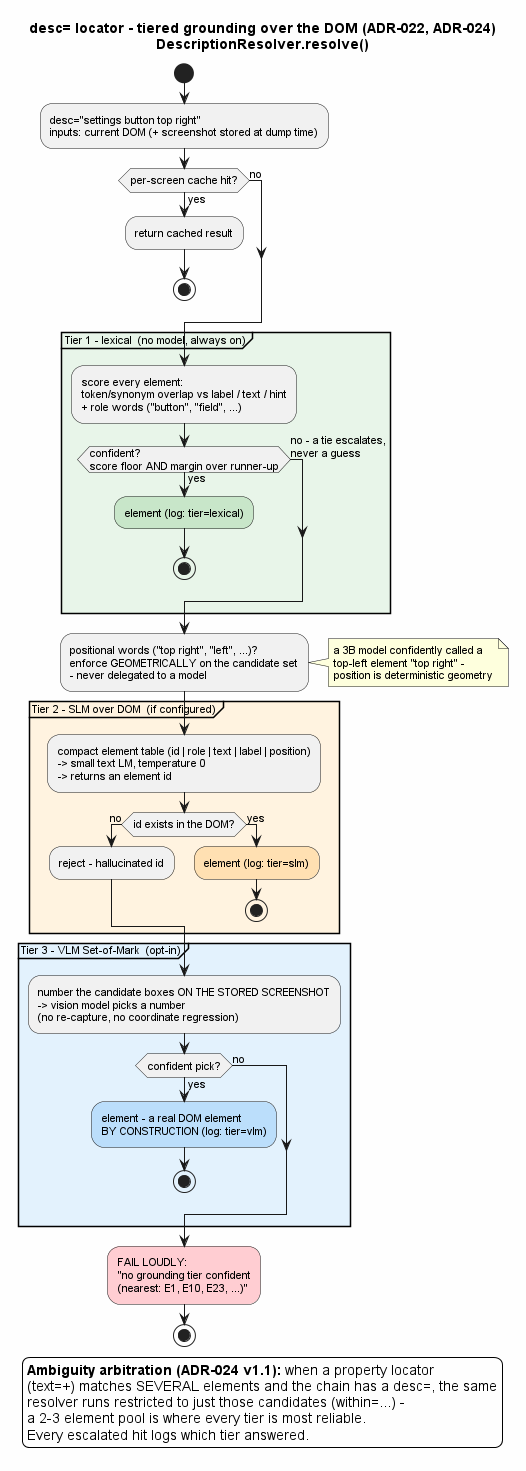
\includegraphics[width=0.62\linewidth]{Desc_Grounding.png}
  \caption{Grounding phân tầng cho locator \code{desc=} (ADR-022). Mỗi tier rẻ
  hơn và có tính quyết định cao hơn tier tiếp theo; nếu có nhiều candidate ngang
  nhau, hệ thống \emph{chuyển lên tier tiếp theo} thay vì đoán. Các từ chỉ vị trí
  được áp dụng bằng geometry trước khi gọi model; id do model hallucinate sẽ bị
  kiểm tra và loại bỏ dựa trên DOM; còn VLM tier trả về một phần tử DOM theo thiết
  kế nhờ Set-of-Mark trên screenshot đã lưu. Cùng resolver này, khi bị giới hạn
  trong tập candidate mơ hồ, cũng được dùng để phân xử các property locator trùng
  khớp nhiều phần tử (ADR-024).}
  \label{fig:descgrounding}
\end{figure}

\subsection{Môi trường kỹ thuật}
Hệ thống chạy trên Python~3.9 với bản build PyTorch hỗ trợ CUDA; môi trường được quản
lý bằng \code{uv}. Quá trình phát triển diễn ra sau corporate proxy chặn các public
code host, và điều này ảnh hưởng đến một số quyết định: code mô hình bên ngoài được
vendor và pin bằng setup script thay vì tải dưới dạng submodule; trang tài liệu
render toàn bộ UML diagram offline bằng renderer cục bộ. Các công cụ hỗ trợ gồm
PyQt5 Visual DOM Viewer (capture, inspect, export), Streamlit dashboard và công cụ
annotation.

% =====================================================================
\section{Đánh giá}
\label{sec:eval}
% =====================================================================

\subsection{Phương pháp đánh giá}
Chất lượng được đánh giá theo bốn trục bằng evaluation harness:
\begin{itemize}[leftmargin=1.4em]
  \item \textbf{Phát hiện phần tử}: precision, recall, F1 và mean IoU so với
        bounding box ground truth đã annotation;
  \item \textbf{OCR}: độ chính xác ký tự và tỷ lệ lỗi ký tự/từ (CER/WER);
  \item \textbf{Hierarchy}: độ đúng của containment và liên kết label; và
  \item \textbf{Chất lượng locator}: tính duy nhất và độ ổn định của locator được
        sinh ra.
\end{itemize}
Benchmark sử dụng \textbf{dataset UI tổng hợp} (ảnh chụp màn hình được sinh bằng
chương trình ở độ phân giải $1920\times1080$, có ground truth chính xác --- bounds,
\code{visual\_type}, text và containment --- theo cùng schema mà pipeline sinh ra),
được chia thành 167 ảnh huấn luyện và \textbf{44 ảnh kiểm thử}. Prediction là danh
sách phần tử pipeline sinh cho từng ảnh kiểm thử; matching được thực hiện theo
phương pháp greedy dựa trên IoU với threshold 0.5. Do ground truth chỉ là danh sách
phần tử phẳng có tham chiếu parent (không phải cây lồng nhau) và không chứa locator,
báo cáo này chỉ trình bày hai trục element detection và OCR; các trục hierarchy và
locator cần ground truth có cây/locator và được dành cho dataset annotation trong
tương lai. Tất cả số liệu được tính bởi evaluation harness của dự án
(\code{visual\_dom.evaluation}).

\subsection{Xây dựng và tăng cường dataset}
Không có benchmark công khai nào trực tiếp nhắm tới bối cảnh của VizDOM --- các
GUI được render tùy biến hoặc được quan sát qua camera, đồng thời có ground truth
có cấu trúc. Vì vậy, dataset được chính dự án tạo ra theo ba lớp bổ trợ lẫn nhau,
cân bằng giữa quy mô, tính đa dạng và mức độ sát với kênh thu nhận thực tế.

\paragraph{Tổng hợp bằng chương trình (benchmark có nhãn).} Các template UI có thể
tham số hóa (login, dashboard, \dots) được render với nhiều theme sáng/tối và độ
phân giải khác nhau. Mỗi lần render đồng thời sinh ra ảnh chụp màn hình
\emph{cùng với} ground truth chính xác (bounds phần tử,
\code{visual\_type}, text và containment) theo chính schema của pipeline. Cách này
tạo được nhãn không nhiễu ở quy mô lớn mà không cần annotation thủ công --- bao
gồm phép chia 167/44 ảnh train/test được sử dụng ở trên --- nên được chọn làm
benchmark có thể tái lập.

\paragraph{Layout do LLM thiết kế (tính đa dạng).} Các template viết thủ công
thường đơn điệu về mặt thị giác, vì vậy một mô hình ngôn ngữ lớn (Claude) được sử
dụng như một \emph{UI designer}: khi được prompt về một lớp ứng dụng, chẳng hạn
màn hình thông tin--giải trí trên ô tô, mô hình đề xuất một layout cụ thể để
renderer chuyển thành ảnh chụp màn hình kèm ground truth tương ứng. Cách làm này
bổ sung tính đa dạng về cấu trúc --- các nhóm control không thông thường và widget
đặc thù miền ứng dụng --- mà template cố định khó bao phủ, trong khi chi phí gán
nhãn gần như không đáng kể.

\paragraph{Tăng cường mô phỏng camera (domain robustness).} Do một động lực trung
tâm của dự án là đọc màn hình \emph{qua camera}, các ảnh chụp màn hình sạch được
tăng cường để mô phỏng kênh này: perspective warp (góc nhìn lệch trục), kết hợp
với glare, blur và sensor noise, với một hoặc nhiều biến thể cho mỗi ảnh. Ground
truth vẫn được giữ lại --- chính xác đối với các hiệu ứng photometric và vẫn hợp
lệ trong trường hợp perspective, vì VizDOM trước tiên hiệu chỉnh vùng màn hình đã
phát hiện về góc nhìn chính diện rồi mới chạy detection. Tập dữ liệu này kiểm tra
trực tiếp đường xử lý screen rectification và tạo áp lực lên đặc trưng khác biệt
cốt lõi của VizDOM: hoạt động khi không có accessibility tree.

Ba lớp trên kết hợp quy mô có nhãn với chi phí thấp (synthesis), tính đa dạng cấu
trúc (LLM design) và độ sát với kênh thu nhận thực tế (augmentation). Phép chia
dataset tổng hợp là benchmark có thể tái lập; còn các lớp LLM và camera được dùng
để hỗ trợ phát triển và đánh giá robustness, mở rộng độ bao phủ về phía điều kiện
triển khai thực tế. Vì vậy, các điểm số tuyệt đối trong phần này được báo cáo trên
tập tổng hợp sạch; các lớp LLM và camera không thuộc benchmark được chấm điểm, và
việc xây dựng một tập dữ liệu thực tế lớn hơn có nhãn vẫn là hướng phát triển trong
tương lai.

\subsection{Xác minh chức năng}
Hệ thống đầu-cuối và các dịch vụ phân tán đã được xác minh về mặt chức năng:
\begin{itemize}[leftmargin=1.4em]
  \item Pipeline đầy đủ xử lý ảnh UI tham chiếu và sinh ra DOM hợp lệ (hàng chục
        phần tử có role, locator và label);
  \item Dịch vụ gRPC \textbf{detector} nạp warm model một lần và trả detection cho
        remote client;
  \item Dịch vụ gRPC \textbf{capture} trả về ảnh chụp màn hình giống từng pixel cho
        remote client; và
  \item Dịch vụ gRPC \textbf{actuator} tái tạo chính xác action theo tọa độ chuẩn
        hóa, ánh xạ sang tọa độ thiết bị ở phía server (được xác minh đầu-cuối bằng
        recording actuator và robot-arm homography stub).
\end{itemize}

\subsection{Kết quả định lượng trên benchmark tổng hợp}
Bảng~\ref{tab:results} trình bày metric tổng thể (pooled) cho element detection và
OCR trên tập kiểm thử tổng hợp gồm 44 ảnh; Bảng~\ref{tab:pertype} phân rã recall theo
từng loại phần tử --- có ý nghĩa hơn nhiều đối với kiểm thử --- dưới hai góc nhìn:
overlap nghiêm ngặt (IoU $\geq 0.5$) và \emph{khả năng trở thành mục tiêu click}
(``center-hit'': bounding box dự đoán có chứa tâm phần tử hay không, nghĩa là bài
kiểm thử có thể click vào phần tử hay không).

\begin{table}[H]
  \centering
  \caption{Kết quả tổng thể về element detection và OCR trên tập kiểm thử tổng hợp
  (44 ảnh, IoU threshold 0.5, greedy matching, pooled trên toàn bộ phần tử). Giá trị
  càng cao càng tốt.}
  \label{tab:results}
  \begin{tabular}{lccccc}
    \toprule
    Detector & Precision & Recall & F1 & mIoU & Độ chính xác ký tự \\
    \midrule
    UIED (CPU)   & 0.39 & \textbf{0.71} & 0.51 & 0.68 & 0.92 \\
    OmniParser   & \textbf{0.56} & 0.59 & \textbf{0.58} & \textbf{0.67} & \textbf{0.95} \\
    YOLO         & \multicolumn{5}{c}{\emph{chưa đánh giá --- chưa có weight được huấn luyện cho các lớp UI này}} \\
    \bottomrule
  \end{tabular}
\end{table}

\begin{table}[H]
  \centering
  \caption{Recall theo loại phần tử ground truth dưới hai góc nhìn: overlap nghiêm
  ngặt (IoU$\geq$0.5) và khả năng trở thành mục tiêu click (bounding box dự đoán
  chứa tâm phần tử). ``n'' = số lượng trong tập kiểm thử 44 ảnh. Actionable = button
  + input + checkbox + icon.}
  \label{tab:pertype}
  \begin{tabular}{lc cc cc}
    \toprule
    & & \multicolumn{2}{c}{UIED} & \multicolumn{2}{c}{OmniParser} \\
    \cmidrule(lr){3-4}\cmidrule(lr){5-6}
    GT type & n & IoU$\geq$0.5 & center-hit & IoU$\geq$0.5 & center-hit \\
    \midrule
    button       & 183  & 0.82 & 0.96 & \textbf{1.00} & \textbf{1.00} \\
    input\_field & 135  & 0.95 & 0.99 & \textbf{0.99} & 0.99 \\
    checkbox     & 76   & \textbf{0.68} & 0.82 & 0.20 & \textbf{0.87} \\
    icon         & 36   & 0.08 & 0.28 & \textbf{0.67} & \textbf{1.00} \\
    text         & 1074 & \textbf{0.79} & \textbf{0.99} & 0.59 & 0.98 \\
    block        & 51   & 0.55 & 0.63 & 0.37 & 0.43 \\
    divider      & 145  & 0.00 & 0.10 & 0.00 & 0.21 \\
    \midrule
    actionable (pooled) & 430 & 0.77 & 0.89 & \textbf{0.83} & \textbf{0.97} \\
    \bottomrule
  \end{tabular}
\end{table}

Xét tổng thể, hai backend khá gần nhau (F1 0.51 so với 0.58), nhưng phân tích theo
từng type cho thấy mỗi backend dẫn đầu ở những loại phần tử khác nhau.
\textbf{OmniParser mạnh hơn trên các actionable control mà bài kiểm thử cần thao
tác}: nó định vị \emph{button} hoàn hảo (recall 1.00), \emph{input field} đạt 0.99
và \emph{icon} đạt 0.67 (so với 0.08 của UIED), với bounding box chặt (mIoU 0.68)
--- phù hợp với quan sát thủ công rằng bounding của OmniParser chính xác hơn.
\textbf{UIED tốt hơn với checkbox} (IoU 0.68 so với 0.20) và recall của \emph{text}
(0.79 so với 0.59). Xét khả năng click, cả hai đều mạnh; OmniParser gần như hoàn hảo
trên tập actionable (0.97 pooled; button/icon 1.00, input 0.99), so với 0.89 của
UIED. IoU thấp của OmniParser trên checkbox (0.20) nhưng center-hit cao (0.87) là
ảnh hưởng quen thuộc của quy ước bounding box --- mô hình bao quanh glyph dấu check
thay vì toàn bộ control có padding --- nên phần tử vẫn click được dù strict overlap
thấp.

Hai điểm sau khép lại vòng lặp với quan sát định tính. Thứ nhất, điểm yếu trước đây
trong \emph{classification} (OmniParser gán mọi thứ thành \code{text}/\code{icon})
đã được xử lý: backend hiện suy luận \code{button} / \code{input\_field} /
\code{checkbox} / \code{icon} từ interactivity và geometry có xét độ phân giải, vì
vậy DOM có thể được lớp kiểm thử sử dụng trực tiếp. Thứ hai, trong bối cảnh kiểm thử
GUI --- nơi phần tử chủ yếu cần được \emph{click} một cách tin cậy --- OmniParser là
lựa chọn mặc định mạnh hơn trên benchmark này, còn UIED vẫn là baseline không cần
GPU và phù hợp hơn khi recall text hoặc checkbox là ưu tiên. Các giới hạn cần lưu ý:
đây là tập \emph{tổng hợp, sạch} (điểm tuyệt đối sẽ khác trên UI thực tế); OCR
ensemble không tạo khác biệt đo được ở đây (OCR nội bộ của OmniParser đã thu được
text); và biến thể có SLM refinement chưa được benchmark do cần một dịch vụ Ollama
đang chạy.

\subsection{Cải thiện phân loại loại phần tử của OmniParser}
Đánh giá và kiểm tra thủ công cho thấy một hạn chế độc lập với chất lượng bounding
box: mặc dù \emph{box} của OmniParser chính xác, integration ban đầu ánh xạ mọi
detection thành \code{text} hoặc \code{icon}. Vì vậy, DOM không có role
\code{button} / \code{input\_field} / \code{checkbox} --- độ chính xác phân loại
type trên actionable control bằng \textbf{0\%} theo thiết kế, và logic kiểm thử dựa
trên role không thể sử dụng OmniParser DOM.

Ánh xạ cải tiến (\code{\_infer\_visual\_type}) kết hợp ba tín hiệu. Thứ nhất,
\emph{geometry}: bounding box rộng với chiều cao tương đương ô nhập được xem là
input field, còn bounding box vuông nhỏ được xem là control glyph. Thứ hai,
\emph{width/aspect} phân biệt button với icon --- button rộng hơn rõ rệt (median
width đo được xấp xỉ $2\times$ icon), vì vậy bounding box rộng có label được xem là
button, còn phần tử nhỏ gần vuông là icon. Thứ ba, \emph{caption} của OmniParser
phân biệt checkbox với icon (cả hai đều là hình vuông nhỏ): caption chứa ``check'',
``toggle'', ``radio'' hoặc ``switch'' được đánh dấu là checkbox. Ngoài ra, pipeline
hiện tự động resolve đường dẫn model của OmniParser, vì trước đây một path bị thiếu
có thể âm thầm làm lần chạy suy giảm thành chỉ còn OCR.

Bảng~\ref{tab:typeacc} trình bày hiệu quả qua hai giai đoạn cải tiến đã đo. Ánh xạ
ban đầu chỉ đạt độ chính xác type trên actionable là 0.09 --- đúng duy nhất ở icon,
nhưng kết quả này có được một cách hiển nhiên do \emph{mọi thứ} đều bị gán
\code{icon} (vì vậy không thể nhận diện bất kỳ role nào khác). \emph{Bản sửa đầu
tiên} bổ sung suy luận role dựa trên interactivity và geometry (chiều cao input,
width/aspect), khôi phục button (0.91) và input field (0.99), nâng độ chính xác
actionable lên 0.73 --- nhưng lại \emph{làm giảm} icon: luật geometry phân loại các
glyph vuông nhỏ thành button hoặc checkbox, khiến độ chính xác icon giảm từ mức
1.00 hiển nhiên xuống 0.00; checkbox vẫn gần bằng không (0.12) vì về geometry chúng
khó phân biệt với icon. Việc bổ sung \emph{caption} của OmniParser để phân biệt
checkbox, cùng với tinh chỉnh lại ranh giới width/aspect giữa button và icon, tạo ra
ánh xạ hiện tại: icon phục hồi lên 0.89, checkbox lên 0.55, button giữ ở 0.89 và độ
chính xác actionable đạt \textbf{0.87}. OmniParser DOM hiện có thể được lớp kiểm thử
sử dụng trực tiếp trên tất cả interactive role.

\begin{table}[H]
  \centering
  \caption{Độ chính xác phân loại type trên các actionable control đã matching qua
  hai giai đoạn cải tiến (OmniParser, tập kiểm thử tổng hợp): \emph{trước đây}
  (chỉ text/icon), \emph{bản sửa đầu tiên} (interactivity + geometry) và \emph{hiện
  tại} (+ caption disambiguation và tinh chỉnh lại width/aspect). Khả năng
  localisation (Bảng~\ref{tab:pertype}) không thay đổi --- bảng này chỉ đo
  \emph{type}. $^\dagger$Ánh xạ ban đầu gán mọi non-text thành \code{icon}, vì vậy
  icon đúng một cách hiển nhiên trong khi mọi role khác đều bằng 0.}
  \label{tab:typeacc}
  \begin{tabular}{lccc}
    \toprule
    GT type & Trước đây & Bản sửa đầu tiên & Hiện tại \\
    \midrule
    button       & 0.00 & 0.91 & 0.89 \\
    input\_field & 0.00 & 0.99 & 0.99 \\
    checkbox     & 0.00 & 0.12 & 0.55 \\
    icon         & 1.00$^\dagger$ & 0.00 & \textbf{0.89} \\
    \midrule
    actionable   & 0.09 & 0.73 & \textbf{0.87} \\
    \bottomrule
  \end{tabular}
\end{table}

Checkbox vẫn là role yếu nhất (0.55): chỉ được khôi phục khi caption của OmniParser
đủ đặc trưng (``Checkmark'', ``Toggle''), trong khi nhiều phần tử có caption chung
chung hoặc caption chính là label hiển thị. Việc sử dụng text label liền kề hoặc
caption semantics phong phú hơn để nhận diện checkbox được dành cho future work.


\subsection{Đánh giá định tính trên một ứng dụng thực tế}
\label{sec:realapp}
Benchmark tổng hợp đo được khả năng localisation và phân loại type, nhưng chưa phản
ánh đầy đủ cách các stage tương tác trên một màn hình doanh nghiệp thực tế có mật
độ phần tử cao. Để khảo sát vấn đề này, một ứng dụng dạng client-management console
($980\times562$) được phân tích bằng bốn tổ hợp detector/OCR; các lỗi được phân nhóm
theo loại (Bảng~\ref{tab:combos}). Đây là một nghiên cứu \emph{định tính} --- màn
hình này chưa có ground truth --- nên kết quả được trình bày dưới dạng các nhóm lỗi
quan sát được, không phải điểm số.

\begin{table}[H]
  \centering\footnotesize
  \caption{Các nhóm lỗi quan sát được với từng tổ hợp detector/OCR trên một ứng
  dụng thực tế. ``$\checkmark$'' = không quan sát thấy lỗi thuộc nhóm tương ứng.}
  \label{tab:combos}
  \begin{tabular}{@{}p{4.5cm}p{2.2cm}p{2.2cm}p{2.4cm}p{2.2cm}@{}}
    \toprule
    Tổ hợp & Icon & Nút dạng tile & Text trạng thái nhỏ & Link cuối màn hình \\
    \midrule
    UIED + EasyOCR & Bỏ sót một số & $\checkmark$ & $\checkmark$ & Bị gộp thành một \\
    OmniParser + EasyOCR \emph{(trước khi sửa)} & $\checkmark$ & Bị tách thành 2--3 phần & Bỏ sót nhiều dòng & $\checkmark$ \\
    OmniParser + Tesseract & $\checkmark$ & $\checkmark$ & Bỏ sót nhiều dòng & $\checkmark$ \\
    \textbf{OmniParser + EasyOCR \emph{(sau khi sửa)}} & $\checkmark$ & $\checkmark$ & $\checkmark$ & $\checkmark$ \\
    \bottomrule
  \end{tabular}
\end{table}

Hai trong ba nhóm lỗi thực chất nằm trong pipeline của dự án và chỉ lộ ra khi so
sánh nhiều tổ hợp. Thứ nhất, các dòng trạng thái nhỏ (``Active'', ``Inactive'',
``Low Protection'') biến mất dù baseline cổ điển vẫn đọc được. OCR ensemble
(Section~\ref{sec:impl}) trước đây chỉ \emph{bù chỗ trống}: thêm box từ OCR có
upscaling tại những nơi OmniParser chưa trả kết quả. Khi OCR nội bộ của OmniParser
đã tạo một kết quả rác trong box rất nhỏ (``\textasciitilde ctive'' thay vì
``Active'', cao 8\,px), kết quả tốt hơn từ OCR có upscaling bị loại vì được xem là
trùng; box nhỏ sau đó lại bị minimum-size filter xóa, khiến cả dòng biến mất. OCR
ensemble hiện dùng cơ chế \emph{prefer-external union}: box từ OCR bên ngoài sẽ
\emph{thay thế} box OmniParser mà nó overlap, vì lượt OCR có upscaling được thiết
kế để cung cấp kết quả chất lượng cao hơn.

Thứ hai, các nút tile có caption gồm hai từ (``Check Now'') bị tách thành hai nửa.
Nguyên nhân là splitter dựa trên luật chia mọi control chứa từ hai OCR box trở lên,
trong khi EasyOCR trả box theo \emph{từng từ} còn Tesseract trả một box cho cả dòng.
Đây cũng là lý do lỗi chỉ xuất hiện với một OCR engine. Splitter hiện không chia
control mà detector đã đánh dấu là một phần tử tương tác duy nhất; trong các trường
hợp còn lại, việc tách chỉ xảy ra khi có khoảng cách thực sự đủ lớn
($\geq 1.5\times$ median text height) giữa các đoạn text. Một quan sát độc lập khác
là OCR engine được cấu hình nhưng chưa cài đặt trước đây có thể âm thầm khiến lần
chạy suy giảm về OCR nội bộ của detector; trường hợp này hiện fail fast kèm hướng
dẫn cài đặt.

Sau các bản sửa, OmniParser + EasyOCR không còn lỗi ở cả bốn nhóm trên màn hình thử
nghiệm, trở thành tổ hợp được khuyến nghị rõ ràng; đồng thời không gây regression
trên benchmark tổng hợp hay các phép thử với ứng dụng máy tính. Hai bài học có thể
khái quát: metrics theo từng type trên dữ liệu tổng hợp không phát hiện được lỗi do
sự tương tác giữa các stage, và khả năng hoán đổi cả detector lẫn OCR engine chính
là điều giúp các lỗi này được tìm thấy.

\subsection{Các khía cạnh hiệu năng}
Hiệu năng được phân tích theo ba trục. Số liệu wall-clock cần chờ benchmark so sánh
đồng nhất (Bảng~\ref{tab:results}), vì vậy phần thảo luận này tập trung vào cấu trúc
và dựa trên đặc điểm mô hình đã công bố thay vì timing chưa được đo.

\paragraph{Yêu cầu phần cứng.} Các mô hình grounding lớn và phụ thuộc GPU ---
Aria-UI kích hoạt 3.9B parameter, còn ELAM-7B và Jedi-7B thuộc nhóm 7B --- trong khi
backend UIED của VizDOM chỉ cần CPU. Một đường chạy CPU là khác biệt thực sự đối với
test rig và thiết bị nhúng không có GPU; backend OmniParser chính xác nhưng nặng
được cung cấp cho các host có GPU.

\paragraph{Hiệu quả tái sử dụng.} Parser phân bổ chi phí theo nhiều lần sử dụng: một
lần parse DOM phục vụ nhiều truy vấn locator và assertion ($O(1)$ lần chạy mô hình,
sau đó là $n$ truy vấn cây rẻ), trong khi grounder phải infer lại theo từng
instruction ($n$ lần gọi mô hình). Trong regression suite gồm hàng nghìn bước, khác
biệt tiệm cận này quyết định một công cụ có thực tế hay không --- đây là lập luận
hiệu năng quan trọng cho abstraction DOM trong kiểm thử, độc lập với bất kỳ con số
latency riêng lẻ nào.

\paragraph{Dịch vụ warm-model và offload.} Dịch vụ detector nạp mô hình một lần và
chỉ chạy inference cho các request tiếp theo; một GPU host có thể phục vụ cả nhóm
client CPU nhẹ. Đặt capture trên thiết bị, inference trên GPU host và orchestration
trên client giúp mỗi node đảm nhiệm phần việc phù hợp, đồng thời tránh phải cài mô
hình nặng trên mọi máy. Benchmark dự kiến sẽ báo cáo latency CPU so với GPU và
throughput của detector theo phương pháp đã nêu.

% =====================================================================
\section{Thảo luận và giới hạn}
% =====================================================================
\begin{itemize}[leftmargin=1.4em]
  \item \textbf{Độ bền vững trong thế giới thực.} Detection và nhận diện symbol
        hoạt động tốt trên UI sạch và tổng hợp nhưng yếu hơn với ứng dụng dùng nhiều
        gradient và theme; việc giảm over-segmentation vẫn đang được tiếp tục.
  \item \textbf{Đánh giá định lượng.} Kết quả hiện được báo cáo trên benchmark tổng
        hợp (Phần~\ref{sec:eval}); vẫn cần một tập gán nhãn \emph{thực tế} lớn hơn
        để xác nhận các số liệu có chuyển giao ra ngoài UI sạch hay không, đồng thời
        đánh giá các trục hierarchy và locator mà ground truth hiện tại chưa hỗ trợ.
  \item \textbf{Calibration cho actuation vật lý.} Trường hợp cánh tay robot yêu cầu
        calibration từ ảnh sang không gian vật lý cho từng setup; kiến trúc đã cô
        lập phần này vào plugin nhưng đây vẫn là công việc thực tế, và actuation vật
        lý đi kèm nghĩa vụ an toàn (giới hạn vùng làm việc, e-stop) mà plugin phải
        thực thi.
  \item \textbf{Bảo mật của khả năng mở rộng.} Plugin auto-discovery import code của
        người dùng và channel gRPC hiện chưa có authentication; hai điểm này chấp
        nhận được trong môi trường tin cậy/LAN nhưng đã được đánh dấu cần hardening
        (entry-point discovery, TLS).
\end{itemize}

% =====================================================================
\section{Kết luận và hướng phát triển}
% =====================================================================
VizDOM chứng minh rằng một DOM tương tự UI Automator và có thể sử dụng trong thực tế
có thể được tái dựng từ ảnh chụp màn hình bằng cách kết hợp computer vision cổ điển,
mô hình vision grounding hiện đại và giai đoạn tinh chỉnh bằng mô hình nhỏ; đồng
thời engine này có thể được triển khai linh hoạt nhờ kiến trúc lục giác hướng dịch
vụ. Hệ thống đã mang lại giá trị cho một test framework thực tế và hỗ trợ các cách
triển khai khác thường như capture bằng camera kết hợp actuation bằng cánh tay robot.
Các hướng phát triển tiếp theo gồm: hoàn thiện benchmark định lượng trên dataset gán
nhãn lớn hơn; giảm over-segmentation trên UI thực tế có theme; đánh giá các mô hình
instruction grounding (Aria-UI, ELAM-7B, Jedi) như phương án thay thế hoặc bổ sung
cho bước tinh chỉnh bằng mô hình nhỏ; và hardening dịch vụ bằng authentication/TLS
cùng cơ chế plugin discovery dựa trên setuptools entry point.

\bibliographystyle{plain}
\bibliography{references}

\end{document}
